\documentclass{article}
\usepackage[UTF8]{ctex} % 用于中文排版
\usepackage{geometry}
\usepackage{indentfirst}
\usepackage{enumitem}

\usepackage{titling}    % 用于自定义标题页
\usepackage{graphicx}
\usepackage{float}

\usepackage{xcolor}
\usepackage{listings}

\usepackage{setspace}

% 页面几何设置
\geometry{a4paper, left=25mm, right=25mm, top=25mm, bottom=25mm}
% 取消首行缩进
\setlength{\parindent}{0pt}
% 行间距设置
\setstretch{1.5}
% 自定义字体大小
\newcommand{\fourhao}{\fontsize{14pt}{\baselineskip}\selectfont} % 四号字体
\newcommand{\xiaosihao}{\fontsize{12pt}{\baselineskip}\selectfont} % 小四号字体
\newcommand{\song}{\CJKfamily{song}}
% 设置代码块格式
\lstset{
    basicstyle = \footnotesize\ttfamily,                 % 设置行距,字体
    numbers = left,                                      % 在左侧显示行号
    numberstyle = \tiny \color{gray},                    % 设定行号格式
    keywordstyle = \bfseries \color[RGB]{40,40,255},     % 设定关键字颜色
    numberstyle = \footnotesize \color{darkgray},           
    commentstyle = \color[RGB]{0,96,96},                 % 设置代码注释的格式
    stringstyle = \color[RGB]{128,0,0},                  % 设置字符串格式
    frame = single,                                      % 不显示背景边框
    backgroundcolor = \color[RGB]{245,245,244},          % 设定背景颜色
    language=Verilog                                     % 设置语言
}
\raggedbottom   % 段落间留白, 避免排版时自动拉伸导致的行间距变化。
\begin{document}

% 封面页面
\begin{titlepage}
    \centering
    \vspace*{2cm}

    \Huge
    \textbf{课程名称:EDA 技术综合设计}

    \vspace{3cm}

    \LARGE
    实验名称: 实验八\ 创新设计\\
    基于串口的数字滤波器设计和硬件验证平台

    \vspace{5cm}

    \centering
    \section*{团队成员}
    \Large
    \begin{tabular}{| l | l | l |}
        \hline
        \textbf{姓名} & \textbf{班级} & \textbf{学号} \\ 
        \hline
        王峤宇 & 通信214 & 214022 \\ 
        \hline
        朱书硕 & 通信214 & 214026 \\ 
        \hline
        王占同 & 通信214 & 214010 \\ 
        \hline
    \end{tabular}
    \vfill

    \vspace{1cm}
\end{titlepage}

\newpage
% 第一部分
\section*{\fourhao 一、设计内容及原理}
\xiaosihao
\setstretch{1.5}
% 设计项目内容及设计原理,如真值表、状态表及状态转换图、文字说明等。
数字滤波器从实现结构上划分,有FIR和IIR两种。FIR (Finite Impulse Response)滤波器的特点是它的冲击响应是有限的,它跟过去的信号无关,所以在使用时容易实现,速度快。本次任务为设计一
个 FIR 滤波器。
\subsection*{FIR滤波器原理}
FIR滤波器简单来说, 其本质上就是加权有限数量输入信号的过去值, 来计算当前的输出, 
比如针对按键的消抖, 采样多次值, 由过去判断当前输出, 本质上就是一种滤波器, 但是按键消抖是一种中值滤波器。\\
FIR的基本原理由如下公式给出:
\begin{equation}
    y[n] = \sum_{k=0}^{N-1} h[k] \cdot x[n-k]
\end{equation}
其中, 
\begin{itemize}
    \item $y[n]$ 是输出信号。
    \item $x[n]$ 是输入信号。
    \item $h[k]$ 是滤波器的脉冲响应系数。
    \item $N$ 是滤波器的长度(系数的数量)。
\end{itemize}

线性相位FIR滤波器的关键在于其脉冲响应 $h[k]$ 的对称性。这种对称性可以保证滤波器具有线性相位特性。
根据对称性的不同,可以将线性相位FIR滤波器分为以下两种类型:
\begin{enumerate}
    \item 偶对称FIR滤波器, 第一类线性相位
    \begin{equation}
    h[k] = h[N-1-k]
    \end{equation}
    
    \item 奇对称FIR滤波器, 第二类线性相位
    \begin{equation}
    h[k] = -h[N-1-k]
    \end{equation}
\end{enumerate}
实际应用中, 通常采用第一类线性相位, 便于运算的同时, 其相位特性也是严格不失真的。
\subsection*{线性相位FIR滤波器结构}
FIR的设计通常借助其对称的特性简化设计, 由于对称性的存在,可以减少乘法运算的数量。
例如,对于一个长度为 $N$ 的对称FIR滤波器,只需要将输入数据相加, 采用$\frac{N}{2}$的乘法器, 将其与FIR系数相乘再相加就可以。
\subsection*{串行和并行设计思路}
\subsubsection*{并行设计}
在FPGA设计中,为了提高计算效率,通常会采用并行和流水线结构。通过并行处理多个乘法和加法操作,可以加快滤波器的处理速度。
同时,通过流水线技术,可以将计算过程分解为多个阶段,每个阶段独立完成部分计算,从而提高整体计算效率。\\
\subsubsection*{串行设计}
在FPGA中实现FIR滤波器时,可以采用串行设计方法。这种方法的主要特点是每个时钟周期只处理一个输入数据,
通过多个时钟周期完成整个FIR滤波器的计算。串行设计的主要优点是硬件资源需求较少,但处理速度较慢。
串行FIR滤波器的基本结构如下:
\begin{itemize}
    \item \textbf{移位寄存器}:用于存储输入信号的过去值。每个时钟周期,新的输入样本被移入寄存器,而最旧的样本被移出。
    \item \textbf{乘法器}:用于将输入样本与滤波器系数相乘。由于是串行结构,通常只有一个乘法器,每个时钟周期进行一次乘法运算。
    \item \textbf{累加器}:用于累加乘法器的输出。累加器的结果在每个时钟周期更新,直到所有系数都计算完毕,得到最终的滤波器输出。
\end{itemize}
\subsection*{基础任务}
\textbf{设计任务}:利用板卡资源,设计一个8阶的FIR低通滤波器,采样频率是5KHz,阻带截止频率是 1KHz.具体频率可以板卡实际资源为
参照进行调整。
\begin{figure}[htbp]
    \centering
    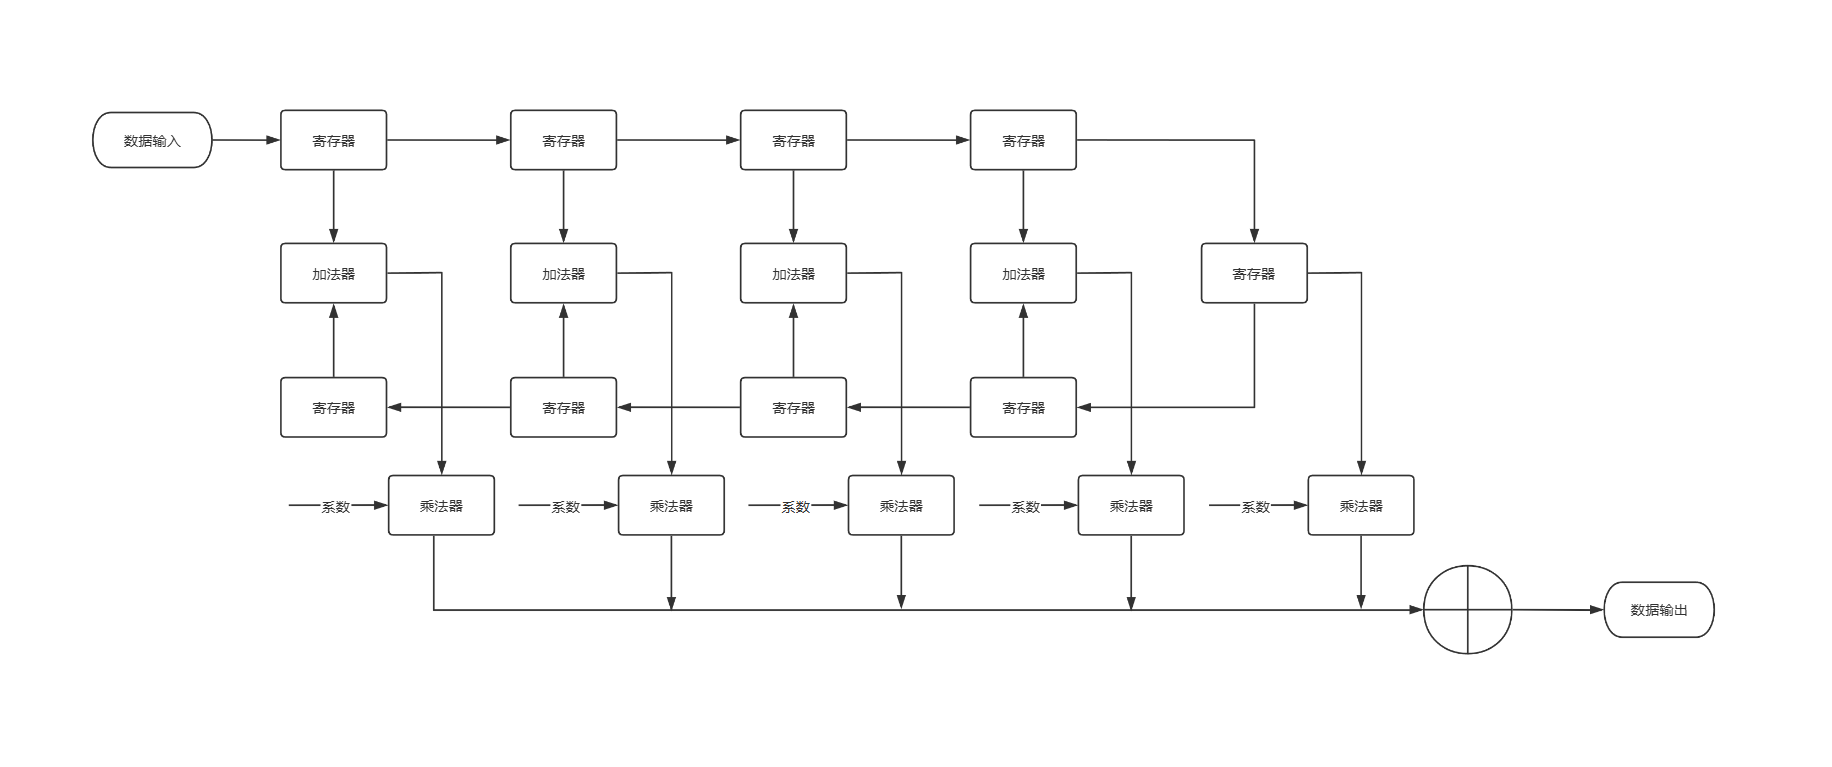
\includegraphics[width=0.7\textwidth]{image/2024-06-28-11-13-34.png}
    \caption{8阶并行FIR滤波器的模块框图}
    \label{image_principle_base_1}
\end{figure}
基于并行结构设计的FIR的8阶数字滤波器模块框图如图\ref{image_principle_base_1}所示。
\subsection*{提高内容}
\textbf{设计任务}:在基础任务的基础上,设置任意阶 FIR 滤波器,要求采用模块化设计思想设计。
\begin{figure}[htbp]
    \centering
    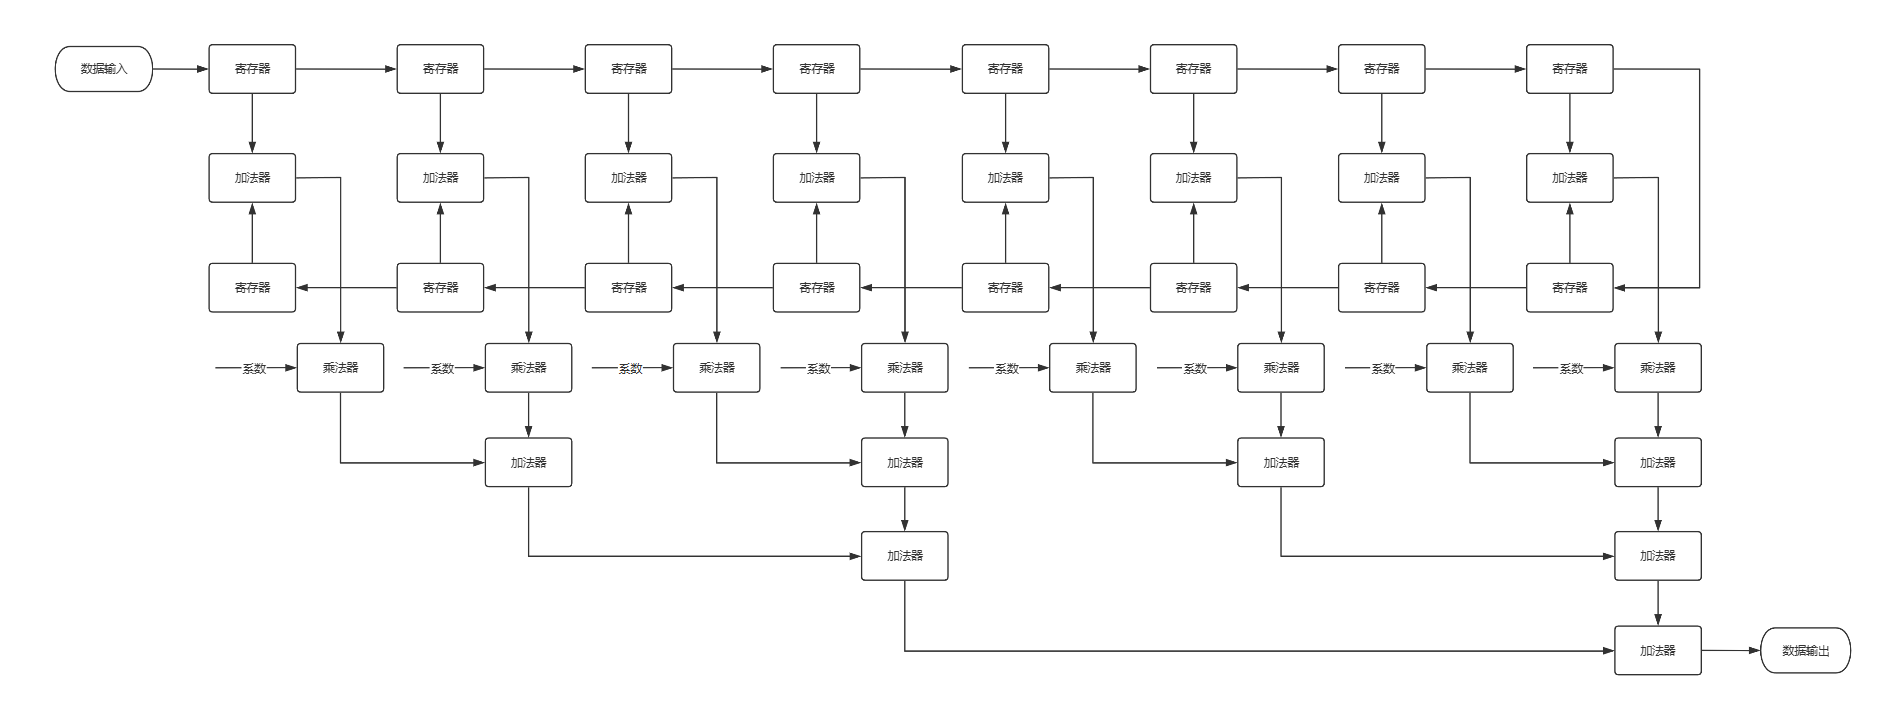
\includegraphics[width=0.7\textwidth]{image/2024-06-28-11-13-08.png}
    \caption{15阶并行FIR滤波器模块框图}
    \label{image_principle_improve_1}
\end{figure}
15阶并行FIR滤波器的模块框图如图\ref{image_principle_improve_1}所示。
\subsection*{拓展任务}
\textbf{任务要求}:滤波器的架构方法可采用串行、并行等不同方法来实现,采用不同方法设计实现FIR滤波器。
\begin{figure}[htbp]
    \centering
    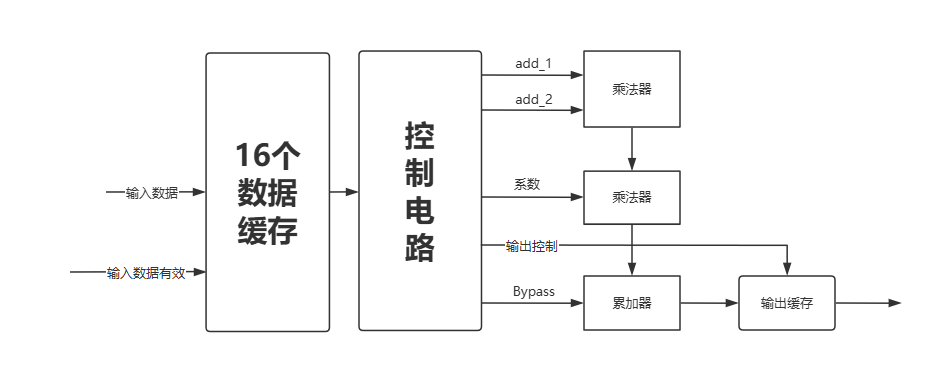
\includegraphics[width=0.7\textwidth]{image/2024-06-28-11-11-33.png}
    \caption{15阶串行FIR滤波器模块框图}
    \label{image_principle_extend_1}
\end{figure}
基于串行结构设计的15阶FIR滤波器的模块框图如图\ref{image_principle_extend_1}所示。
\subsection*{创新设计}
\textbf{设计思路}:不满足仅仅在仿真中实现的FIR滤波器, 将搭建的FIR滤波器综合并部署到FPGA开发板上, 
利用串口与FPGA通信, PC机向FPGA传输待滤波数据, FPGA将滤波输出结果回传到FPGA上,PC通过MATLAB或其
他语言对数据进行验证。\\

\textbf{十六倍过采样原理}:标准UART的RXD前端有一个"1到0跳变检测器",当其连续接受到8个RXD上的地电平时,
该检测器就认为RXD线出现了起始位,进入接受数据状态.在接受状态,接受控制器对数据位7,8,9三个脉冲采样,并遵从
三中取二的原则确定最终值.采用这一方法的根本目的还是为了增强抗干扰,提高数据传送的可靠性,采样信号总是在每
个接受位的中间位置,可以避开数据位两端的边沿失真,也可以防止接受时钟频率和发送时钟频率不完全同步引起的误差.\\

十六倍过采样本身也是对UART这种异步通信的一个延迟补偿, 如果没有过采样的话, 发送端和接收端的时钟将会0~1个
波特率时钟周期, 引入16倍过采样后, 检测到发送的的起始位后, 实现时钟同步, 由于同步的过程由16倍过采样的时钟
控制, 同步之后的时钟相差仅为0~1/16个波特率时钟周期。\\
\begin{figure}[htbp]
    \centering
    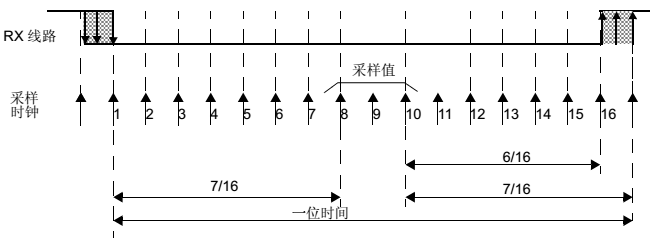
\includegraphics[width=0.7\textwidth]{image/2024-06-27-22-04-57.png}
    \caption{十六倍过采样示意图}
    \label{image_design_innovation_1}
\end{figure}
十六倍过采样的示意图如图\ref{image_design_innovation_1}所示。

\begin{figure}[H]
    \centering
    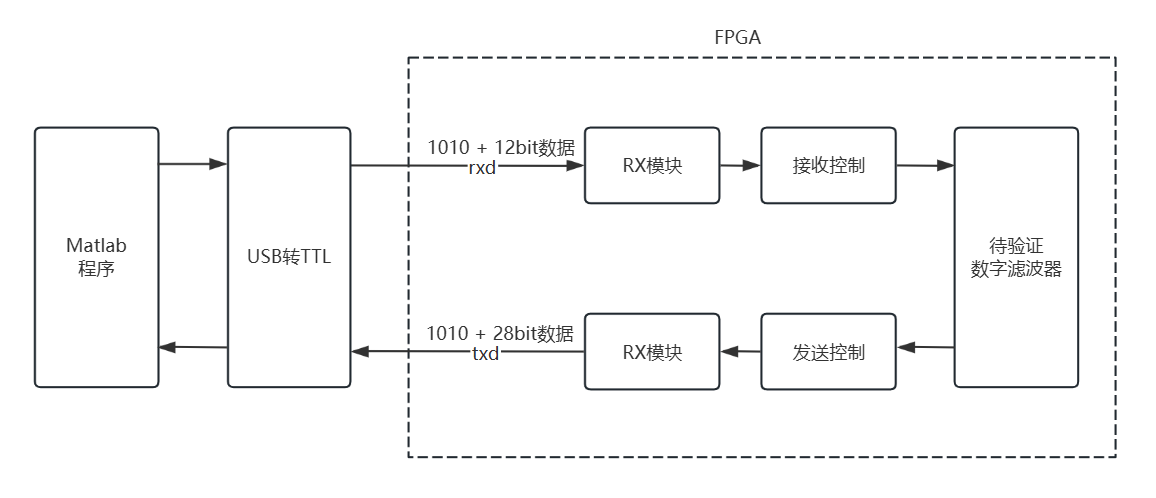
\includegraphics[width=0.7\textwidth]{image/2024-06-29-22-29-18.png}
    \caption{创新设计的模块框图}
    \label{image_design_innovation_2}
\end{figure}
该部分的模块框图如图\ref{image_design_innovation_2}所示, 主要由待验证FIR和串口模块以及相应的控制电路构成, 
上位机部分通过Matlab程序完成串口通信, 直接利用FPGA进行滤波然后检验数据正确性。

% 第二部分
\section*{\fourhao 二、设计过程}
\xiaosihao
\setstretch{1.5}
% 从工程建立开始,一直到硬件调试。
% 按照基础任务、提高任务和拓展任务分别给出相应的源文件、仿真文件、约束文件
\subsection*{基础任务}
并行设计, 使用Xilinx提供的IP核进行设计,源文件如下:
\begin{lstlisting}[language=Verilog, caption={并行八阶FIR滤波器}]
/* 8阶并行FIR滤波器 */
module fir_parallel (
        input rst,           // 复位,低有效
        input clk,           // 工作频率,即采样频率
        input en,            // 输入数据开始信号
        input [11:0]  xin,   // 输入混合频率的信号数据
        output out_rdy,      /* 输出数据有效 */
        output [28:0]  yout  // 输出数据
    );
    /* 滤波器设计 */
    parameter ORDER = 8;                /* 默认为N为偶数 */
    parameter MULT_NUM = ORDER/2 + 1;   /* 系数为奇数 */
    parameter DATA_NUM = (ORDER+1);     /* 系数为奇数 */

    wire signed [11:0] coe[MULT_NUM-1:0];
    assign coe[0] = 12'd60;
    assign coe[1] = 12'd165;
    assign coe[2] = 12'd307;
    assign coe[3] = 12'd432;
    assign coe[4] = 12'd482;

    //(0) 输入数据有效缓存, 保证输入数据延迟5个时钟时输出
    reg [4:0] en_r;
    always @(posedge clk or posedge rst) begin
        if (rst) begin
            en_r[4:0] <= 'b0;
        end
        else begin
            en_r[4:0] <= {en_r[3:0], en};
        end
    end

    //(1) 读取数据
    reg signed [11:0] xin_reg[DATA_NUM-1:0];
    integer i, j;
    always @(posedge clk or posedge rst) begin
        if (rst) begin
            for (i = 0; i < DATA_NUM; i = i+1) begin
                xin_reg[i]  <= 12'b0;
            end
        end
        else if (en) begin
            xin_reg[0] <= xin;
            for (j = 0; j < DATA_NUM - 1; j = j+1) begin
                xin_reg[j+1] <= xin_reg[j]; //周期性移位操作
            end
        end
    end

    //(2) 首尾相加, 实现线性相位结构, 延迟两个时钟
    wire signed [12:0] add_reg[MULT_NUM-1:0];
    genvar l;
    generate
        for (l = 0; l < DATA_NUM/2; l = l+1) begin
            c_addsub_0 your_instance_name (
                .A(xin_reg[l]),             // 首部数据
                .B(xin_reg[DATA_NUM-1-l]),  // 尾部数据
                .CLK(clk),                  // 输入时钟
                .S(add_reg[l])              // 输出数据
            );
        end
    endgenerate

    /* 人为延迟两个周期 */
    reg signed [12:0] add_reg_r[1:0];
    assign add_reg[MULT_NUM-1] = add_reg_r[1];
    always @(posedge clk or posedge rst) begin
        if (rst) begin
            add_reg_r[0] <= 'b0;
            add_reg_r[1] <= 'b0;
        end
        else if(en_r[3]) begin
            add_reg_r[0] <= {xin_reg[MULT_NUM-1][11], xin_reg[MULT_NUM-1]};
            add_reg_r[1] <= add_reg_r[0];
        end
    end

    // (3) 乘法器, 延迟3个时钟
    wire signed [24:0] mout[MULT_NUM-1:0];
    genvar k;
    generate
        for (k=0; k < MULT_NUM; k=k+1) begin
            mult_gen_0 mult_parallel (
                .CLK(clk),          // 时钟
                .A(add_reg[k]),     // 13位的有符号数据
                .B(coe[k]),         // 12位的有符号系数
                .P(mout[k])         // 25位的输出数据
            );
        end
    endgenerate
    
    //(4) 积分累加,MULT_NUM组25bit数据
    reg signed [28:0] sum;
    always @(posedge clk or posedge rst) begin
        if (rst) begin
            sum  <= 29'd0;
        end
        else begin
            sum  <= mout[0] + mout[1] + mout[2] + mout[3] + mout[4];
        end
    end

    reg signed [28:0] yout_r;
    reg out_rdy_r;
    always @(posedge clk or posedge rst) begin
        if (rst) begin
            yout_r <= 29'd0;
        end
        else if (en_r[4]) begin
            yout_r <= sum;
            out_rdy_r <= 1'b1;
        end
        else begin
            out_rdy_r <= 1'b0;
        end
    end
    assign out_rdy = out_rdy_r;
    assign yout  = yout_r;
endmodule
\end{lstlisting}
通过Matlab程序生成用于仿真的数据结果如下:
\begin{lstlisting}[language=Matlab, caption={生成12位的波形数据}]
clear all;close all;clc;

fs = 5e3;
T = 1 / fs;
n = 0:2047;
t = n * T;
x = cos(2*pi*50*t) + 0.5*cos(2*pi*2000*t);
x = mapminmax(x);
x_dis = floor((2 ^ 11 - 1) * x);
fid = fopen('signal_data.txt', 'wt'); %写数据文件
for k=1:2048
    B_si = dec2bin(x_dis(k) + (x_dis(k)<0)*2^12, 12);
    fprintf(fid,'%s\n',B_si);
end
fprintf(fid,';'); 
fclose(fid);
stem(x(1:256));
title('原信号');
\end{lstlisting}
\begin{figure}[htbp]
    \centering
    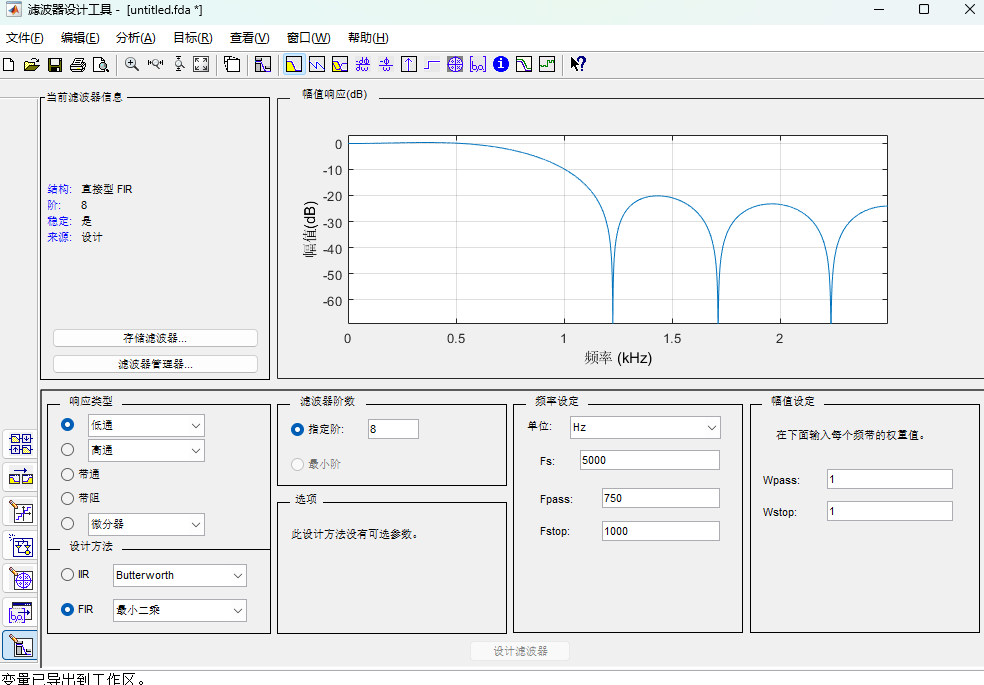
\includegraphics[width=0.7\textwidth]{image/2024-06-28-21-37-14.png}
    \caption{滤波器设计}
    \label{image_design_base_1}
\end{figure}
设计的滤波器如图\ref{image_design_base_1}所示, 采用最小二乘法设计, 阻带权值为40, 通带为1, 
阻带截止频率为1000Hz, 对输入为200Hz+2000Hz的信号进行滤波。
\begin{figure}[H]
    \centering
    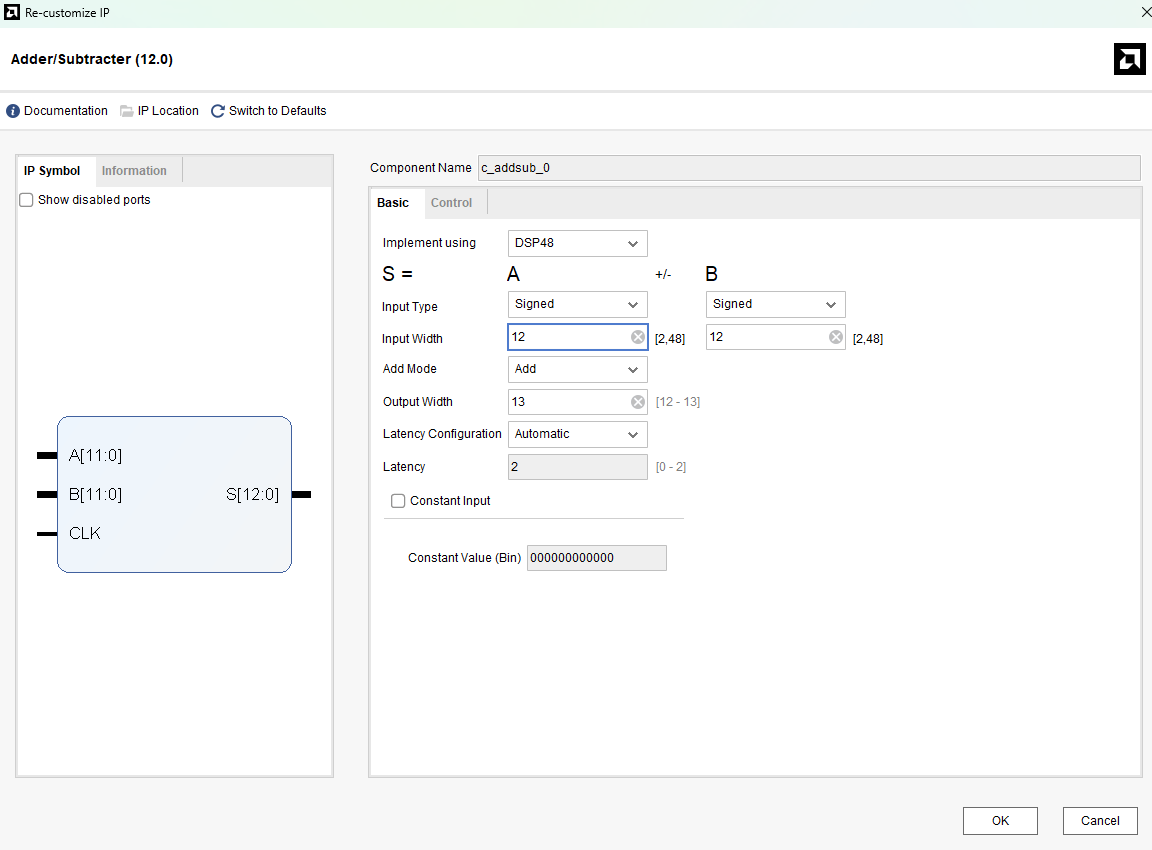
\includegraphics[width=0.7\textwidth]{image/2024-06-26-15-56-44.png}
    \caption{加法器IP}
    \label{image_design_base_2}
\end{figure}
加法器IP核的设置如图\ref{image_design_base_2}所示, 使用Xilinx提供的DSP Slice资源上提供的乘法器和加法器实现。
\begin{figure}[H]
    \begin{minipage}[t]{0.45\linewidth}
        \centering
        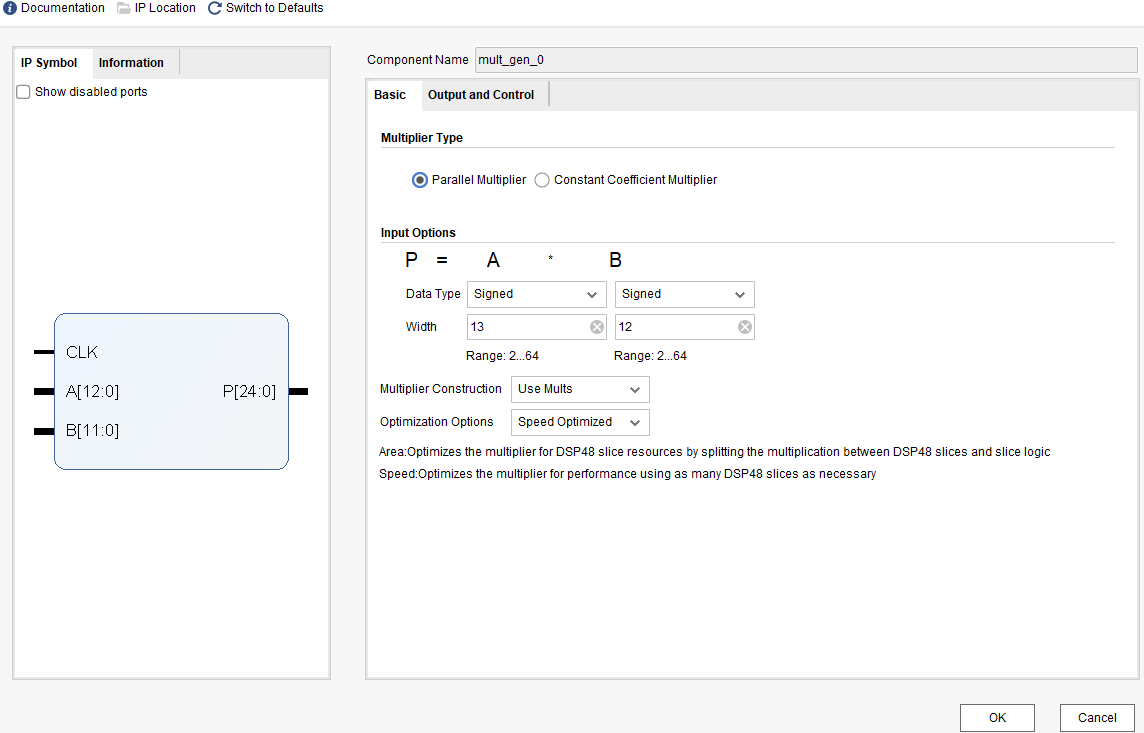
\includegraphics[width=0.7\textwidth]{image/2024-06-26-16-09-08.png}
        \caption{乘法器IP核配置a}
        \label{image_design_base_3_1}
    \end{minipage}
    \begin{minipage}[t]{0.45\linewidth}
        \centering
        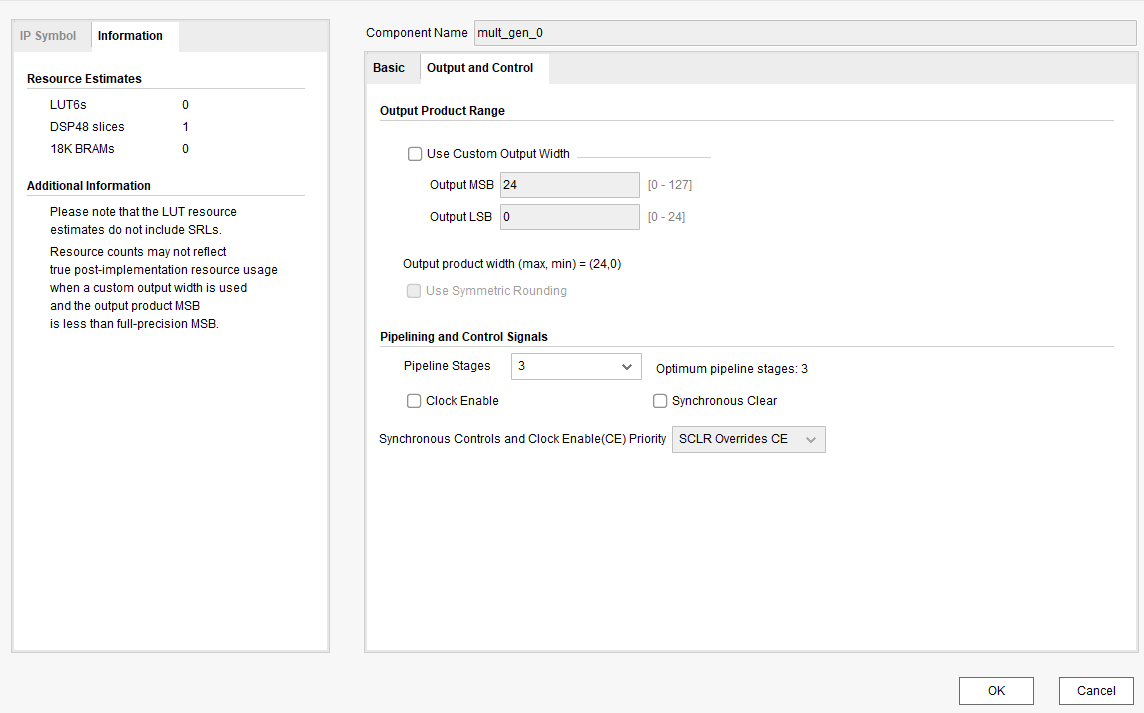
\includegraphics[width=0.7\textwidth]{image/2024-06-26-16-11-08.png}
        \caption{乘法器IP核配置b}
        \label{image_design_base_3_2}
    \end{minipage}
\end{figure}
乘法器的IP核配置结果如图\ref{image_design_base_3_1}和图\ref{image_design_base_3_2}所示, DSP Slice资源提供的乘法器为流水线工作方式, 
配置为13位和12位的符号数输入, 完成两个数据相加后和FIR系数的乘法运算, 在设置流水线阶段时, 设置为系统
提示的最佳阶段, 三段流水线, 输出结果延迟三个时钟。
仿真文件如下文件如下:
\begin{lstlisting}[language=Verilog, caption={8阶FIR滤波器仿真文件}]
module fir_parallel_tb;
    reg  rst;
    reg  clk;
    reg  en;
    reg [11:0] xin;
    wire signed [28:0] yout;
    wire out_rdy;
    parameter SIN_DATA_NUM = 2048;
    parameter FILE_PATH_A = "E:/Projects/matlabProject/fpgaTools/signal_data.txt";
    parameter FILE_PATH_B = "E:/Projects/matlabProject/fpgaTools/signal_res.txt";   
    initial begin
        rst = 0;
        clk = 0;
        #10;
        rst = 1;
        #10;
        rst = 0;
    end

    reg [11:0] stimulus[0: SIN_DATA_NUM-1];
    integer i, j;
    integer file;
    initial begin
        $readmemb(FILE_PATH_A, stimulus);
        file = $fopen(FILE_PATH_B, "w");
        en = 1;
        i = 0;
        j = 0;
        xin = 0;
        #200;
        forever begin
            xin = stimulus[i];
            @(negedge clk) begin
                if (i == SIN_DATA_NUM-1) begin
                    i = 0;
                end
                else begin
                    i = i + 1;
                end
            end
            @(posedge clk) begin
                if (out_rdy) begin
                    $fwrite(file, "%d\n", yout);
                    j = j + 1;
                    if (j == SIN_DATA_NUM) begin
                        $finish;
                        $fclose(file);
                    end
                end
            end
        end
    end
   
    fir_parallel  fir_parallel_inst (
        .rst(rst),
        .clk(clk),
        .en(en),
        .xin(xin),
        .yout(yout),
        .out_rdy(out_rdy)
    );

    always #5  clk = ! clk ;

endmodule
\end{lstlisting}
\subsection*{提高任务}
设计15阶的FIR滤波器, 采样频率16kHz, 输入信号为语音信号, 使用低通滤波器保留3.4kHz以下的信号, 滤除5000hz单频噪声, 并且改善最终计算的求和过程。
改善后的FIR滤波器源文件如下:
\begin{lstlisting}[language=Verilog, caption={15阶并行FIR滤波器}]
/* 16阶并行FIR滤波器 */
module fir_parallel_15 (
        input rst,           // 复位,低有效
        input clk,           // 工作频率,即采样频率
        input en,            // 输入数据开始信号
        input [11:0] xin,    // 输入混合频率的信号数据
        output out_rdy,      // 输出数据有效
        output [27:0] yout   // 输出数据
    );
    /* 滤波器设计 */
    parameter ORDER = 15;               /* 默认N为奇数 */
    parameter MULT_NUM = (ORDER+1)/2;   /* 乘法器个数为偶数 */
    parameter DATA_NUM = (ORDER+1);     /* 数据个数为偶数数 */

    wire signed [11:0] coe[MULT_NUM-1:0];
    assign coe[0] = -12'd94;
    assign coe[1] =  12'd101;
    assign coe[2] =  12'd190;
    assign coe[3] =  12'd75;
    assign coe[4] = -12'd153;
    assign coe[5] = -12'd110;
    assign coe[6] =  12'd362;
    assign coe[7] =  12'd865;

    //(0) 输入数据有效缓存, 保证输入数据延迟5+6个时钟时输出
    reg [10:0] en_r;
    always @(posedge clk or posedge rst) begin
        if (rst) begin
            en_r <= 'b0;
        end
        else begin
            en_r <= {en_r[9:0], en};
        end
    end

    //(1) 读取数据
    reg signed [11:0] xin_reg[DATA_NUM-1:0];
    integer i, j;
    always @(posedge clk or posedge rst) begin
        if (rst) begin
            for (i = 0; i < DATA_NUM; i = i+1) begin
                xin_reg[i]  <= 12'b0;
            end
        end
        else if (en) begin
            xin_reg[0] <= xin;
            for (j = 0; j < DATA_NUM - 1; j = j+1) begin
                xin_reg[j+1] <= xin_reg[j]; //周期性移位操作
            end
        end
    end

    //(2) 首尾相加, 实现线性相位结构, 延迟两个时钟
    wire signed [12:0] add_reg[MULT_NUM-1:0];
    genvar l;
    generate
        for (l = 0; l < DATA_NUM/2; l = l+1) begin
            c_addsub_0 adder_12bit (
                .A(xin_reg[l]),             // 首部数据
                .B(xin_reg[DATA_NUM-1-l]),  // 尾部数据
                .CLK(clk),                  // 输入时钟
                .S(add_reg[l])              // 输出数据
            );
        end
    endgenerate

    // (3) 乘法器, 延迟3个时钟
    wire signed [24:0] mout[MULT_NUM-1:0];
    genvar k;
    generate
        for (k=0; k < MULT_NUM; k=k+1) begin
            mult_gen_0 mult_25bit (
                .CLK(clk),          // 时钟
                .A(add_reg[k]),     // 13位的有符号数据
                .B(coe[k]),         // 12位的有符号系数
                .P(mout[k])         // 25位的输出数据
            );
        end
    endgenerate
    
    //(4) 积分累加,8组25bit数据, 输出28bit数据, 使用三级加法器, 延迟2*3个周期
    wire signed [27:0] sum[6:0];
    genvar m;
    generate
        for (m=0; m < 7; m=m+1) begin
            if (m < 4) begin
                c_addsub_1 adder_28bit (
                    .A({{3{mout[m*2][24]}}, mout[m*2]}),
                    .B({{3{mout[m*2+1][24]}}, mout[m*2+1]}),
                    .CLK(clk),
                    .S(sum[m])
                );
            end
            else begin
                c_addsub_1 adder_28bit (
                    .A(sum[(m-4)*2]),
                    .B(sum[(m-4)*2+1]),
                    .CLK(clk),
                    .S(sum[m])
                );
            end
        end
    endgenerate
    reg signed [27:0] yout_r;
    reg out_rdy_r;
    always @(posedge clk or posedge rst) begin
        if (rst) begin
            yout_r <= 28'd0;
        end
        else if (en_r[10]) begin
            yout_r <= sum[6];
            out_rdy_r <= 1'b1;
        end
        else begin
            out_rdy_r <= 1'b0;
        end
    end
    assign out_rdy = out_rdy_r;
    assign yout = yout_r;
endmodule
\end{lstlisting}
针对15阶的FIR滤波器的仿真文件如下:
\begin{lstlisting}[language=Verilog, caption={15阶并行FIR滤波器的仿真文件}]
module fir_parallel_15_tb;
    reg  rst;
    reg  clk;
    reg  en;
    reg [11:0] xin;
    wire signed [28:0] yout;
    wire out_rdy;
    parameter SIN_DATA_NUM = 2048;
    parameter FILE_PATH_A = "E:/Projects/matlabProject/fpgaTools/signal_data.txt";
    parameter FILE_PATH_B = "E:/Projects/matlabProject/fpgaTools/signal_res.txt";   
    initial begin
        rst = 0;
        clk = 0;
        #10;
        rst = 1;
        #10;
        rst = 0;
    end

    reg [11:0] stimulus[0: SIN_DATA_NUM-1];
    integer i, j;
    integer file;
    initial begin
        $readmemb(FILE_PATH_A, stimulus);
        file = $fopen(FILE_PATH_B, "w");
        en = 1;
        i = 0;
        j = 0;
        xin = 0;
        #200;
        forever begin
            xin = stimulus[i];
            @(negedge clk) begin
                if (i == SIN_DATA_NUM-1) begin
                    i = 0;
                end
                else begin
                    i = i + 1;
                end
            end
            @(posedge clk) begin
                if (out_rdy) begin
                    $fwrite(file, "%d\n", yout);
                    j = j + 1;
                    if (j == SIN_DATA_NUM) begin
                        $finish;
                        $fclose(file);
                    end
                end
            end
        end
    end
   
    fir_parallel_15 fir_parallel_inst (
        .rst(rst),
        .clk(clk),
        .en(en),
        .xin(xin),
        .yout(yout),
        .out_rdy(out_rdy)
    );

    always #5  clk = ! clk ;

endmodule
\end{lstlisting}
语音信号的matlab文件如下:
\begin{lstlisting}[language=Matlab, caption={语音信号文件处理}]
clear all; clc; close all;

[file, path]  = uigetfile('*.wav');     % 读取音频
[xx, fs] = audioread([path, file]);     % 读取音频

xx=xx-mean(xx);                         % 消除直流分量
x=xx/max(abs(xx));                      % 幅值归一化
N=length(x);                            % 计算音频长度

time=(0:N-1)/fs;                        % 计算时间
noiseFreq=5000;                         % 单频噪声频率
noiseAmp=0.125;                         % 单频噪声幅度
signal=x + noiseAmp*cos(2*pi*noiseFreq*time)'; % 添加噪声
res = mapminmax(signal);
x_dis = floor((2 ^ 11 - 1) * res);
fid = fopen('signal_data.txt', 'wt'); %写数据文件
for k=1:N
    B_si = dec2bin(x_dis(k) + (x_dis(k)<0)*2^12, 12);
    fprintf(fid, '%s\n', B_si);
end
fprintf(fid,';'); 
fclose(fid);

% 作图
subplot 411; plot(time,x,'k'); grid;
title('原始语音'); ylabel('幅值'); xlabel('时间/s');

subplot 412; audioFFT = fft(x);
plot((0:round(N/2)-1) / N * fs, abs(audioFFT(1:round(N/2)) / N), 'k');grid;
title('原始语音频谱'); ylabel('幅值'); xlabel('freq(Hz)');

subplot 413; plot(time,signal,'k');grid;
title('带噪语音'); ylabel('幅值'); xlabel('时间/s');

subplot 414; audioFFT = fft(signal);
plot((0:round(N/2)-1) / N * fs, abs(audioFFT(1:round(N/2)) / N), 'k');grid;
title('带噪语音频谱'); ylabel('幅值'); xlabel('freq(Hz)');    
\end{lstlisting}
\begin{figure}[H]
    \centering
    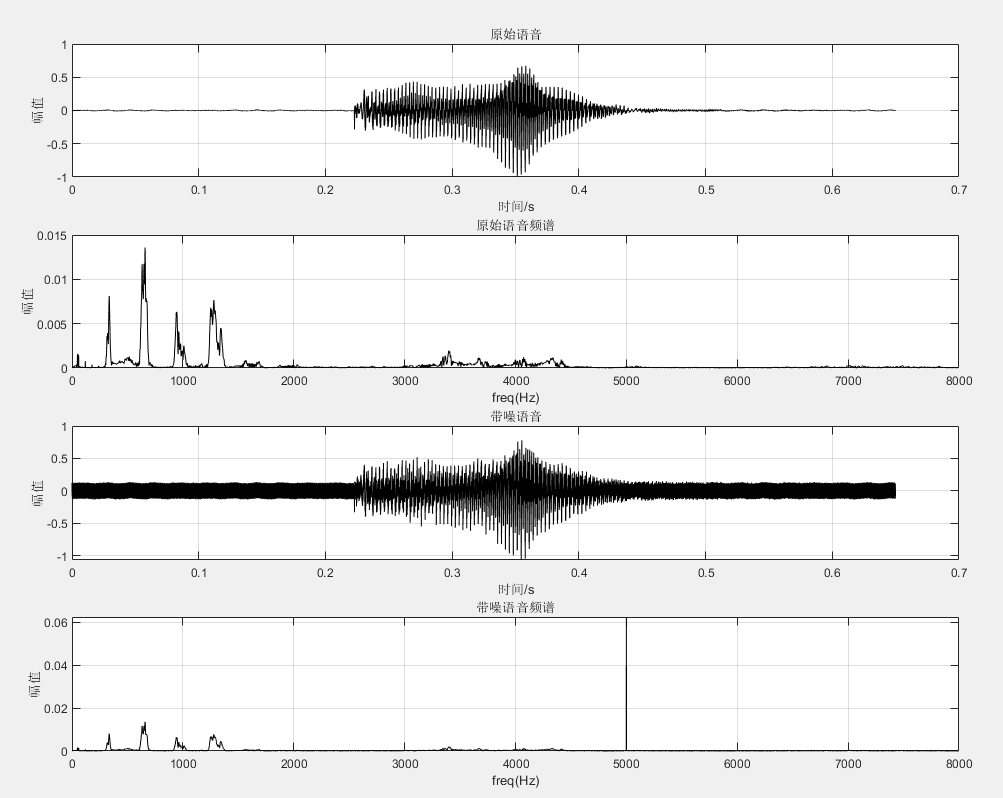
\includegraphics[width=0.7\textwidth]{image/2024-06-26-21-34-18.png}
    \caption{语音信号时域和频域图}
    \label{image_design_improve_1}
\end{figure}
语音信号频谱和时域图如图\ref{image_design_improve_1}所示, 在16000采样速率的语音信号中添加了幅值为0.125单频噪音信号,
并将其转变为12bit的补码输出到txt文件中, 供Verilog仿真的系统级函数\$readmemb读取, 并输入到FIR滤波器之中。
\begin{figure}[H]
    \centering
    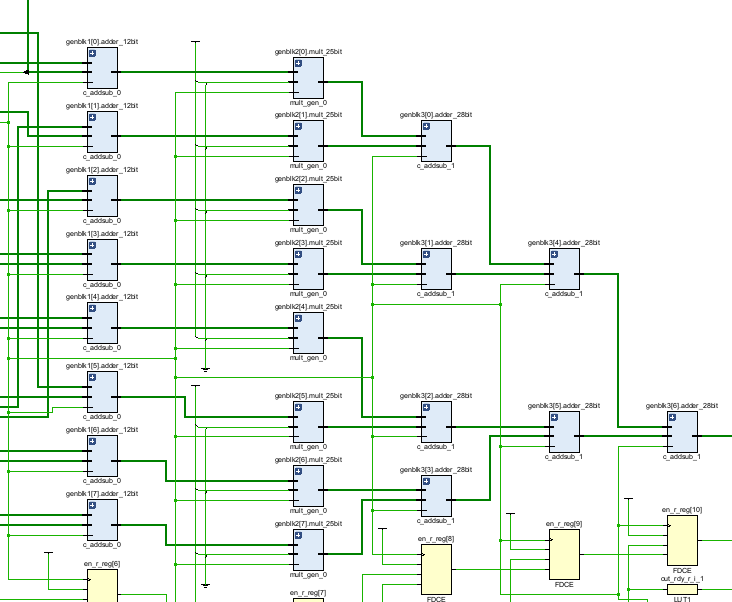
\includegraphics[width=0.7\textwidth]{image/2024-06-27-02-27-52.png}
    \caption{15阶并行FIR滤波器综合结果}
    \label{image_design_improve_2}
\end{figure}
15阶并行FIR滤波器的综合结果如图\ref{image_design_improve_2}所示, 使用了8个乘法器和8+7个加法器, 极大的消耗资源, 但整个系统仅使用到一个LUT。
\subsection*{拓展任务}
15阶串行FIR滤波器源文件如下:
\begin{lstlisting}[language=Verilog, caption={15阶串行FIR滤波器源文件}]
`timescale 1ns / 1ns
/* 串行设计FIR滤波器 */s
module fir_serial (
    input rst,          // 低电平复位
    input clk,          // 系统工作时钟,100MHz
    input en,           // 输入数据有效信号
    input [11:0] xin,   // 输入信号数据
    output out_rdy,       // 输出数据有效信号
    output [27:0] yout  // 输出数据
    );
    // 数据有效缓冲
    reg [15:0] en_r;
    always @ (posedge clk or posedge rst) begin
        if (rst) begin
            en_r[15:0] <= 'b0;
        end
        else begin
            en_r[15:0] <= {en_r[14:0], en};
        end
    end
    
    // 滤波器系数
    wire signed [11:0] coe[7:0];
    assign coe[0] = -12'd94;
    assign coe[1] =  12'd101;
    assign coe[2] =  12'd190;
    assign coe[3] =  12'd75;
    assign coe[4] = -12'd153;
    assign coe[5] = -12'd110;
    assign coe[6] =  12'd362;
    assign coe[7] =  12'd865;

    // (1) 输入数据移位部分
    reg [2:0] cnt;
    always @ (posedge clk or posedge rst) begin
        if (rst) begin
            cnt <= 3'b0;
        end
        else if (en || cnt != 0) begin
            cnt <= cnt + 1'b1;    // 8个周期计数
        end
    end

    // (1) 读入数据, 每8个周期读入一次数据, 延迟一个周期
    integer i, j;
    reg signed [11:0] xin_reg[15:0];
    always @ (posedge clk or posedge rst) begin
        if (rst) begin
            for (i=0; i<16; i=i+1) begin
                xin_reg[i] <= 12'b0;
            end
        end
        else if (cnt == 3'd0 && en) begin       // 每8个周期读入一次有效数据
            xin_reg[0] <= xin;
            for (j=0; j<15; j=j+1) begin
                xin_reg[j+1] <= xin_reg[j];     // 数据移位
            end
        end
    end
    
    /* 3个周期 */
    reg signed [11:0] add_a, add_b;
    wire signed [12:0] add_s;
    reg signed [11:0] coe_s[2:0];
    wire [2:0] xin_index = cnt[2:0] >= 1 ? cnt[2:0] - 1 : 3'd7;
    always @ (posedge clk or posedge rst) begin
        if (rst) begin
            add_a <= 12'b0;
            add_b <= 12'b0;
            coe_s[0] <= 12'b0;
        end
        else if (en_r[xin_index]) begin //from en_r[1]
            add_a <= xin_reg[xin_index];
            add_b <= xin_reg[15-xin_index];
            coe_s[0] <= coe[xin_index];
        end
    end
    always @(posedge clk or posedge rst) begin
        if (rst) begin
            coe_s[1] <= 12'b0;
            coe_s[2] <= 12'b0;
        end
        else begin
            coe_s[1] <= coe_s[0];
            coe_s[2] <= coe_s[1];
        end
    end
    c_addsub_0 adder (
        .A(add_a),
        .B(add_b),
        .CLK(clk),
        .S(add_s)
    );

    // (3) 乘法运算,使用一个流水线乘法器, 3个周期
    wire signed [24:0] mout;
    /* 延迟3个时钟的流水线乘法器 */
    mult_gen_0 mult (
        .CLK(clk),  // input wire CLK
        .A(add_s),  // input wire [12 : 0] A
        .B(coe_s[2]),  // input wire [11 : 0] B
        .P(mout)    // output wire [24 : 0] P
    );

    // (4) 积分累加,延迟2个周期
    wire signed [27:0] sum;
    c_accum_0 your_instance_name (
        .B(mout),          // input wire [24 : 0] B
        .CLK(clk),         // input wire CLK
        .BYPASS(cnt==3'd7),// input wire BYPASS
        .Q(sum)            // output wire [27 : 0] Q
    );
    reg out_rdy_r;
    reg signed [27:0] yout_r;     // 输出数据
    always @(posedge clk) begin
        if (en_r[15]) begin
            out_rdy_r <= 1'b1;
            yout_r <= sum;
        end
        else begin
            out_rdy_r <= 1'b0;
        end
    end
    
    assign yout = yout_r;
    assign out_rdy = out_rdy_r;
endmodule
\end{lstlisting}
15阶串行FIR滤波器的仿真文件如下:
\begin{lstlisting}[language=Verilog, caption={15阶串行FIR滤波器的仿真文件}]
`timescale 1ns / 1ps

module fir_serial_tb;
    //input
    reg clk;
    reg rst;
    reg en ;
    reg [11:0] xin ;
    //output
    wire signed [27:0] yout ;
    wire out_rdy ;
    parameter SIN_DATA_NUM = 10400;

    initial begin
        clk = 1'b0;
        forever begin
            #5 clk = ~clk;
        end
    end
    
    parameter FILE_PATH_A = "E:/Projects/matlabProject/fpgaTools/extend/signal_data.txt";
    parameter FILE_PATH_B = "E:/Projects/matlabProject/fpgaTools/extend/signal_res.txt";

    initial begin
        rst = 1'b1;
        #30 rst = 1'b0;
    end
    reg [11:0] stimulus[0: SIN_DATA_NUM-1];
    integer i, j, file;
    initial begin
        $readmemb(FILE_PATH_A, stimulus);
        file = $fopen(FILE_PATH_B, "w");
        en = 0;
        i = 0;
        j = 0;
        xin = 0;
        #200;
        forever begin
            repeat(7) @(negedge clk); //空置7个周期,每过16个周期给数据
            en = 1;
            xin = stimulus[i];
            @(negedge clk);
            en = 0;         //输入数据有效信号只持续一个周期即可
            if (i == SIN_DATA_NUM-1)
                i = 0;
            else 
                i = i + 1;
        end
    end
    always @(posedge out_rdy) begin
        $fwrite(file, "%d\n", yout);
        j = j + 1;
        if (j == SIN_DATA_NUM) begin
            $finish;
            $fclose(file);
        end
    end
    fir_serial fir_filter_inst (
        .rst(rst),
        .clk(clk),
        .en(en),
        .xin(xin),
        .out_rdy(out_rdy),
        .yout(yout)
    );
endmodule
\end{lstlisting}
\begin{figure}[H]
    \centering
    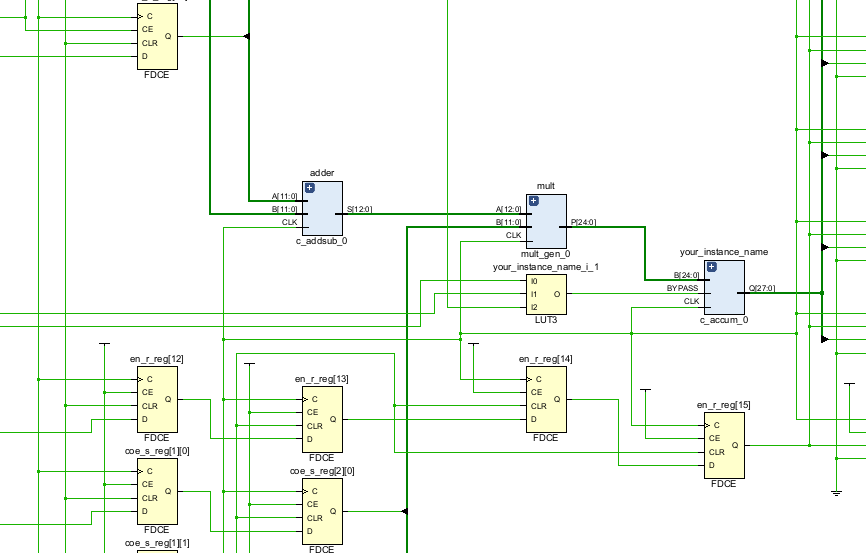
\includegraphics[width=0.7\textwidth]{image/2024-06-27-02-25-16.png}
    \caption{串行FIR综合结果}
    \label{image_design_extend_1}
\end{figure}
15阶串行FIR滤波器的总结结果如图所示\ref{image_design_extend_1}所示, 仅使用了1个加法器、1个乘法器以及一个累加器,
其数据输入要求间隔至少8个周期, 因为流水线以8个周期完成一次计算, 此外其数据相比于并行延迟较多, 同样的DSP单元, 延迟达到了16个周期。 
相比于串行设计用到了大量的查找表和触发器资源, 但也不到片上总资源的\%0.5。
% 第三部分
\subsection*{创新设计}
用到的16倍过采样串口通信模块的源文件如下:
\begin{lstlisting}[language=Verilog, caption={16倍过采样UART模块}]
/* 时钟模块 */
module uart_clk_div (
    input clk,
    input rstn,
    output clk_uart,
    output clk_uart_16
    );
    // localparam step_freq = 32'd6597070;     /* 9600 * 16 */
    localparam step_freq = 32'd79164837;    /* 115200 * 16 */

    reg [31:0] cnt = 32'b0;
    reg cnt_equal;
    always@(posedge clk or negedge rstn) begin
        if(!rstn)
            cnt <= 32'b0;
        else  
            cnt <= cnt + step_freq;
    end
    always @(posedge clk or negedge rstn) begin
        if (!rstn) begin
            cnt_equal <= 1'b0;
        end else if(cnt < 32'h8000_0000) begin
            cnt_equal <= 1'b0;
        end else begin
            cnt_equal <= 1'b1;  
        end
    end
    assign clk_uart_16 = cnt_equal;
    
    /* 16倍分频 */
    reg [3:0] cnt2 = 4'b0;
    always @(posedge clk_uart_16 or negedge rstn) begin
        if (!rstn) begin
            cnt2 <= 4'b0;
        end else begin
            cnt2 <= cnt2 + 1'b1;
        end
    end
    assign clk_uart = cnt2[3];
endmodule
/* 16倍过采样rx模块 */
module uart_rx(
    input rxd,
    input clk_uart_16,
    input rst,
    output rx_ne,
    output reg [7:0] data_i
    );
    reg [7:0] data_i_buf;

    // 接收器三个状态, 格雷码
    localparam st_IDLE = 3'b000;      /* 空闲状态 */
    localparam st_confirm = 3'b001;   /* 确认接收 */
    localparam st_RECEIVE = 3'b011;   /* 接收数据 */
    localparam st_STOP = 3'b010;      /* 等待停止位 */
    localparam st_RXNE = 3'b110;      /* 接收非空 */
    reg [2:0] rx_cur_st, rx_nxt_st;
    reg [3:0] count1;
    reg [3:0] count2;
    /* 状态切换 */
    always @(posedge clk_uart_16 or posedge rst) begin
        if (rst) begin
            rx_cur_st <= st_IDLE;
        end
        else begin
            rx_cur_st <= rx_nxt_st;
        end
    end

    /* 过采样时钟计数 */
    always @(posedge clk_uart_16) begin
        if (rx_cur_st == st_confirm || rx_cur_st == st_RECEIVE) begin
            count2 <= count2 + 1'b1;
        end else begin
            count2 <= 4'b0000;
        end
    end

    reg sampleBuf1;     /* 采样缓存单元 */
    reg sampleBuf2;     /* 采样缓存单元 */
    reg sampleBuf3;     /* 采样缓存单元 */
    always @(posedge clk_uart_16 or posedge rst) begin
        if (rst) begin
            {sampleBuf1, sampleBuf2, sampleBuf3} <= 3'b0;
        end
        else if (rx_cur_st == st_confirm) begin
            if (rxd) begin
                sampleBuf1 <= sampleBuf1 | 1'b1;
            end else begin
                sampleBuf1 <= sampleBuf1;
            end
        end else if (rx_cur_st == st_RECEIVE) begin
            case (count2)
                4'd7: sampleBuf1 <= rxd;
                4'd8: sampleBuf2 <= rxd;
                4'd9: begin
                    casez ({sampleBuf1, sampleBuf2, rxd})
                        3'b11?, 3'b1?1, 3'b?11: begin
                            sampleBuf3 <= 1'b1;
                        end
                        default: sampleBuf3 <= 1'b0;
                    endcase
                end
                default: sampleBuf1 <= sampleBuf1;
            endcase
        end else begin
            sampleBuf1 <= 1'b0;
        end
    end

    always @(posedge clk_uart_16) begin
        if (rx_cur_st == st_RECEIVE) begin
            if (count2 == 4'd10) begin
                count1 <= count1 + 1'b1;
            end else begin
                count1 <= count1;
            end
        end else begin
            count1 <= 4'b0000;
        end
    end

    always @(posedge clk_uart_16 or posedge rst) begin
        if (rst) begin
            data_i_buf <= 8'b0;
        end
        else if (rx_cur_st == st_RECEIVE) begin
            if (count2 == 4'd10) begin
                data_i_buf <= {sampleBuf3, data_i_buf[7:1]};
            end else begin
                data_i_buf <= data_i_buf;
            end
        end
    end

    /* 状态切换 */
    always @(*) begin
        case (rx_cur_st)
            st_IDLE: begin
                if (rxd == 1'b0) begin           /* 接收到开始信号 */
                    rx_nxt_st <= st_confirm;
                end else begin
                    rx_nxt_st <= st_IDLE;
                end
            end
            st_confirm: begin                    /* 确认起始信号 */
                if (count2 == 4'b1000) begin
                    if (!sampleBuf1) begin
                        rx_nxt_st <= st_RECEIVE;
                    end else begin
                        rx_nxt_st <= st_IDLE;
                    end
                end else begin
                    rx_nxt_st <= st_confirm;
                end
            end
            st_RECEIVE: begin                     /* 接收到数据 */
                if (count1 == 4'd9) begin
                    rx_nxt_st <= st_STOP;
                end else begin
                    rx_nxt_st <= st_RECEIVE;
                end
            end
            st_STOP: begin
                if (rxd) begin
                    rx_nxt_st <= st_RXNE;
                end else begin
                    rx_nxt_st <= st_STOP;
                end
            end
            st_RXNE: begin
                if (rxd == 1'b0) begin
                    rx_nxt_st <= st_confirm;
                end else begin
                    rx_nxt_st <= st_IDLE;
                end
            end
            default: rx_nxt_st <= st_IDLE;
        endcase
    end
    always @(posedge rx_ne or posedge rst) begin
        if (rst) begin
            data_i <= 8'b0;
        end
        else begin
            data_i <= data_i_buf;
        end
    end
    /* 接收完成标志位 */
    assign rx_ne = (rx_cur_st == st_RXNE)? 1'b1:1'b0;
endmodule
/* tx模块 */
module uart_tx(
    input [7:0] data_o,
    output reg txd,
    input clk,
    input rst,
    input tx_en
    );
    // 发送机四个状态
    localparam st_IDLE = 2'b00;     /* 空闲状态 */
    localparam st_start = 2'b01;    /* 发送起始位 */
    localparam st_data = 2'b10;     /* 发送数据 */
    localparam st_end = 2'b11;      /* 发送结束 */

    reg [2:0] count;
    reg [1:0] tx_cur_st, tx_nxt_st;
    reg [7:0] data_o_tmp;

    reg tx_en_buf;
    always @(posedge tx_en or posedge clk) begin
        if (tx_en) begin
            tx_en_buf <= 1'b1;
        end else if (tx_cur_st == st_start) begin
            tx_en_buf <= 1'b0;
        end
    end

    always @(*) begin               /* 组合逻辑 */
        case (tx_cur_st)
            st_IDLE: begin
                if (tx_en_buf) begin
                    tx_nxt_st <= st_start;
                end else begin
                    tx_nxt_st <= st_IDLE;
                end
            end
            st_start: begin
                tx_nxt_st <= st_data;
            end
            st_data: begin
                if (count == 7) begin
                    tx_nxt_st <= st_end;
                end else begin
                    tx_nxt_st <= st_data;
                end
            end
            st_end: begin
                if (tx_en_buf) begin
                    tx_nxt_st <= st_start;
                end else begin
                    tx_nxt_st <= st_end;
                end
            end
            default: tx_nxt_st <= st_IDLE;
        endcase
    end

    always @(posedge clk) begin     /* 时序逻辑 */
        if (rst) begin
            tx_cur_st <= st_IDLE;
        end else begin
            tx_cur_st <= tx_nxt_st;
        end
    end
    
    always @(posedge clk) begin
        if (tx_cur_st == st_data) begin
            count <= count + 1'b1;
        end else begin
            count <= 0;
        end
    end

    always @(posedge clk) begin
        if (tx_cur_st == st_start) begin
            data_o_tmp <= data_o;
        end else if (tx_cur_st == st_data) begin
            data_o_tmp <= {1'b0, data_o_tmp[7:1]};
        end
    end

    always @(posedge clk) begin
        if (tx_cur_st == st_start) begin
            txd <= 0;
        end else if (tx_cur_st == st_data) begin
            txd <= data_o_tmp[0];
        end else begin
            txd <= 1;
        end
    end
endmodule
\end{lstlisting}
基于串口通信的FIR硬件验证设计源文件如下:
\begin{lstlisting}[language=Verilog, caption={基于串口FIR硬件验证}]
module fir_top (
    input clk,      /* 100MHz时钟输入 */
    input rxd,      /* rxd接口 */
    output txd,     /* txd接口 */
    input rst       /* 复位信号 */
    );
    // 时钟模块
    wire clk_uart;
    wire clk_uart_16;
    uart_clk_div uart_clk_div (
        .clk(clk),
        .rstn(!rst),
        .clk_uart(clk_uart),
        .clk_uart_16(clk_uart_16)
    );
    // 串口接收模块
    wire [7:0] data_rx;
    wire rx_ne;
    uart_rx uart_rx1 (
        .clk_uart_16(clk_uart_16),
        .rxd(rxd),
        .rst(rst),
        .data_i(data_rx),
        .rx_ne(rx_ne)
    );
    // 串口发送模块
    reg [7:0] data_tx;
    reg tx_en;
    uart_tx uart_tx1 (
        .clk(clk_uart),
        .txd(txd),
        .rst(rst),
        .data_o(data_tx),
        .tx_en(tx_en)
    );
    wire out_rdy;
    wire [27:0] yout;
    reg [11:0] xin;
    reg data_en;
    fir_parallel_15  fir_parallel_15_inst (
        .rst(rst),
        .clk(clk_uart_16),
        .en(data_en),
        .xin(xin),
        .out_rdy(out_rdy),
        .yout(yout)
    );

    /* 一段式状态机 */
    reg cnt_rx;
    always @(posedge clk_uart_16 or posedge rst) begin
        if (rst) begin
            xin <= 12'b0;
            cnt_rx <= 2'b0;
            data_en <= 1'b0;
        end
        else if (cnt_rx == 1'b1) begin
            if (rx_ne) begin
                xin <= {xin[11-:4], data_rx};
                cnt_rx <= 1'b0;
                data_en <= 1'b1;
            end
        end
        else if(rx_ne && data_rx[7:4] == 4'b1010) begin
            xin <= {data_rx[3:0], 8'b0};
            cnt_rx <= 1'b1;
            data_en <= 1'b0;
        end
        else begin
            cnt_rx <= 1'b0;
            data_en <= 1'b0;
        end
    end

    reg [9:0] cnt_tx; /* 2^5 + 2^4 */
    reg cnt_tx_en;
    reg [31:0] data_out_buf;
    always @(posedge clk_uart_16 or posedge rst) begin
        if (rst) begin
            cnt_tx_en <= 1'b0;
            cnt_tx <= 5'b0;
            data_out_buf <= 32'b0;
        end
        else if (out_rdy) begin
            data_out_buf <= {4'b1010, yout};
            cnt_tx_en <= 1'b1;
            cnt_tx <= 10'b1;
        end
        else if (cnt_tx == 10'b0) begin
            cnt_tx_en <= 1'b0;
        end
        else if (cnt_tx_en == 1'b1) begin
            if (cnt_tx[7:0] == 8'b1110_0000) begin
                tx_en <= 1'b1;
                data_tx <= data_out_buf[31-:8];
                data_out_buf <= {data_out_buf[24:0], 8'b0};
            end
            else begin
                tx_en <= 1'b0;
            end
            cnt_tx <= cnt_tx + 5'd1;
        end
    end
endmodule
\end{lstlisting}
基于串口通信的FIR硬件验证设计仿真文件如下:
\begin{lstlisting}[language=Verilog, caption={基于串口FIR硬件验证的仿真文件}]
module fir_top_tb;
    reg  clk;
    wire rxd;
    wire txd;
    reg  rst;
    reg  clk_uart;
    reg  clk_uart_16;
    parameter SIN_DATA_NUM = 10400;
    parameter FILE_PATH_A = "E:/Projects/matlabProject/fpgaTools/innovation/signal_data.txt";
    parameter FILE_PATH_B = "E:/Projects/matlabProject/fpgaTools/innovation/signal_res.txt";   
    /* 复位 */
    initial begin
        rst = 1;
        #30 rst = 0;
    end
    /* 时钟生成 */
    initial begin
        clk = 1'b0;
        forever begin
            #5 clk = ~clk;
        end
    end
    initial begin
        clk_uart_16 = 0;
        forever begin
            #271 clk_uart_16 = ~clk_uart_16;
        end
    end
    initial begin
        clk_uart = 0;
        forever begin
            #4336 clk_uart = ~clk_uart;
        end
    end
    
    fir_top fir_top_inst (
        .clk(clk),
        .rxd(rxd),
        .txd(txd),
        .rst(rst)
    );

    reg  tx_en;
    reg [7:0] data_o;
    uart_tx uart_tx (
        .clk(clk_uart),
        .txd(rxd),
        .rst(rst),
        .data_o(data_o),
        .tx_en(tx_en)
    );
    wire rx_ne;
    wire [7:0] data_i;
    uart_rx uart_rx (
        .rst(rst),
        .clk_uart_16(clk_uart_16),
        .rxd(txd),
        .data_i(data_i),
        .rx_ne(rx_ne)
    );

    reg [11:0] stimulus[0: SIN_DATA_NUM-1];
    integer i;
    initial begin
        $readmemb(FILE_PATH_A, stimulus);
        #100;
        for (i = 0; i<SIN_DATA_NUM; i = i+1) begin
            data_o <= {4'b1010, stimulus[i][11-:4]};
            @(negedge clk_uart) tx_en <= 1'b1;
            @(posedge clk_uart) tx_en <= 1'b0;
            repeat(8)@(posedge clk_uart);
            data_o <= {stimulus[i][7:0]};
            @(negedge clk_uart) tx_en <= 1'b1;
            @(posedge clk_uart) tx_en <= 1'b0;
            repeat(4)@(posedge rx_ne);
        end
    end
    reg signed [27:0] data_rx;
    integer j;
    integer k;
    integer file;
    initial begin
        #100;
        file = $fopen(FILE_PATH_B, "w");
        for (j = 0; j<SIN_DATA_NUM; j = j + 1) begin
            @(posedge rx_ne) data_rx[27:24] = data_i[3:0];
            while (data_i[7:4] != 4'b1010) begin
                @(posedge rx_ne) data_rx[27:24] = data_i[3:0];
            end
            @(posedge rx_ne) data_rx[23:16] = data_i;
            @(posedge rx_ne) data_rx[15:8]  = data_i;
            @(posedge rx_ne) data_rx[7:0]   = data_i;
            $fwrite(file, "%d\n", data_rx);
        end
        $finish;
        $fclose(file);
    end
endmodule
\end{lstlisting}
创新设计部分的约束文件如下:
\begin{lstlisting}[language=Verilog, caption={创新设计部分的约束文件}]
# 100MHz时钟信号
set_property -dict {PACKAGE_PIN P17 IOSTANDARD LVCMOS33} [get_ports clk]
# 复位信号
set_property -dict {PACKAGE_PIN R11 IOSTANDARD LVCMOS33} [get_ports rst]
# 串口
set_property -dict {PACKAGE_PIN N5 IOSTANDARD LVCMOS33} [get_ports rxd]
set_property -dict {PACKAGE_PIN T4 IOSTANDARD LVCMOS33} [get_ports txd]
\end{lstlisting}
\section*{\fourhao 三、仿真结果}
\xiaosihao
\setstretch{1.5}
% 对仿真图像要有解释,要对所有的可能性进行标注及解释
% 按照基础任务、提高任务和拓展任务分别给出仿真结果
\subsection*{基础任务}
\begin{figure}[htbp]
    \centering
    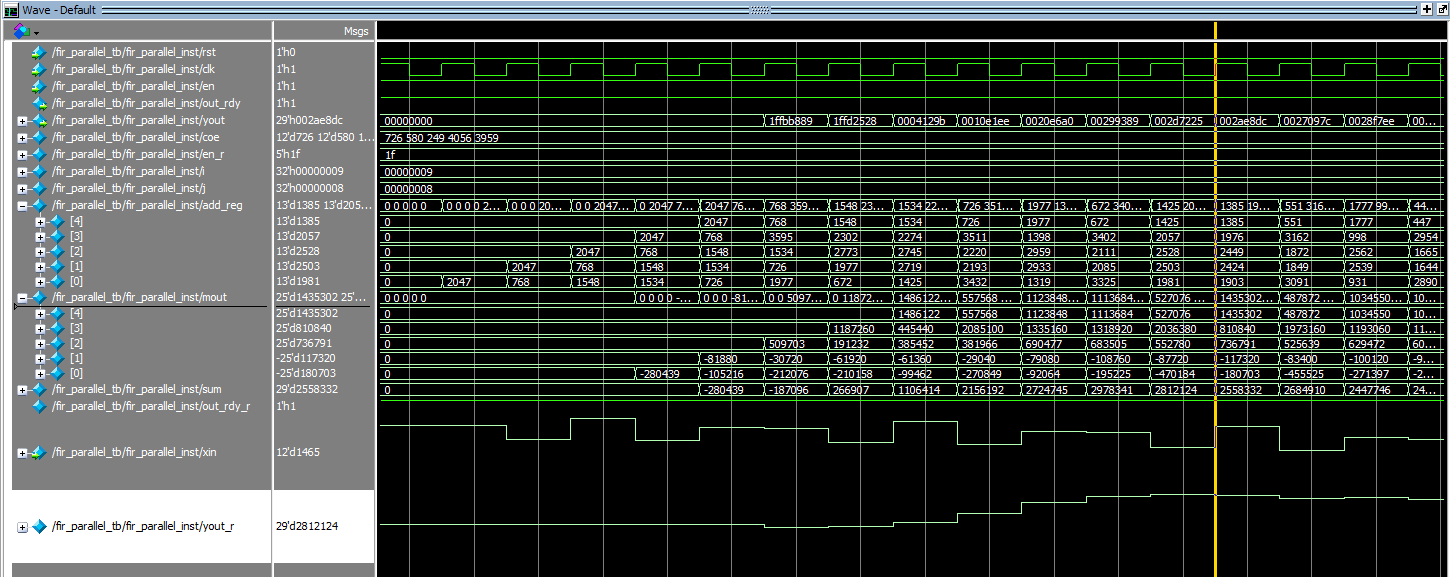
\includegraphics[width=0.7\textwidth]{image/2024-06-28-21-15-02.png}
    \caption{数据流过程仿真}
    \label{image_base_sim_1}
\end{figure}
针对输入数据计算流程的仿真结果如图\ref{image_base_sim_1}所示, 当数据en有效时, 
开始读入xin数据, 数据读入后看以看到, 其在延迟两个时钟后由加法器输出到对应的
add\_reg中, 然后数据开始不为0, 乘法器开始工作, 从add\_reg不为0开始, 延迟3时钟后乘法器开始输出, 再延迟一个时钟, 最后得到累加结果。\\
此后, 流水线进入填满状态, 每一个时钟输出一个有效数据。 
\begin{figure}[H]
    \centering
    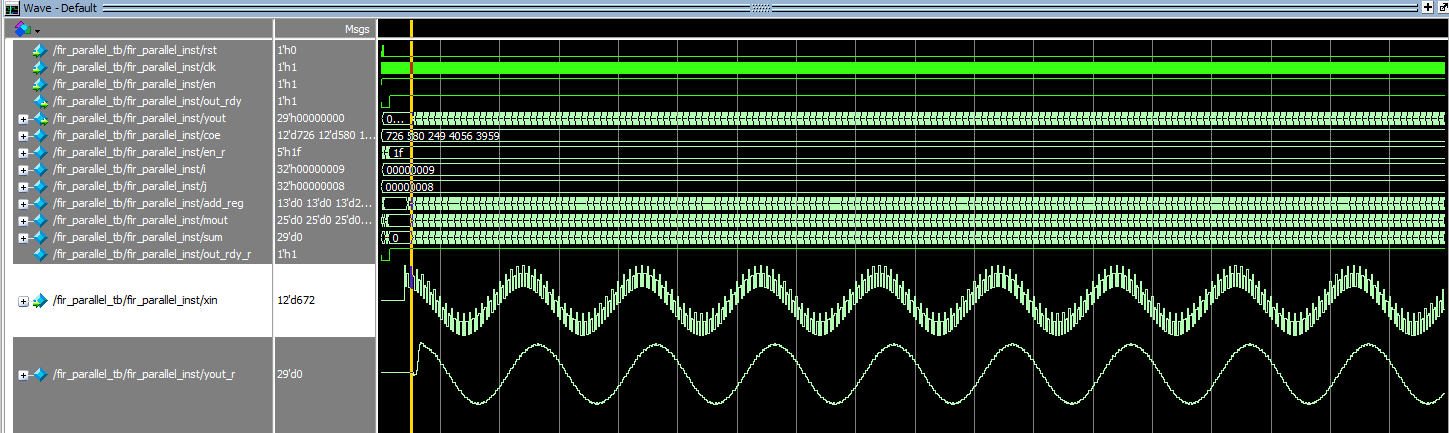
\includegraphics[width=0.7\textwidth]{image/2024-06-28-21-13-57.png}
    \caption{滤波结果仿真}
    \label{image_base_sim_2}
\end{figure}
滤波结果如图\ref{image_base_sim_2}所示, 输入信号如下:
\begin{lstlisting}[language=Matlab]
fs = 5e3;
T = 1 / fs;
n = 0:2047;
t = n * T;
x = cos(2*pi*50*t) + 0.5*cos(2*pi*2000*t);
\end{lstlisting}
将50Hz的信号视为目标信号, 2000Hz的信号视为单频噪声, 可以看到通过1k截止频率的低通FIR滤波器后其信噪比明显得到改善, 2000Hz信号被削弱。
\subsection*{提高任务}
\begin{figure}[H]
    \centering
    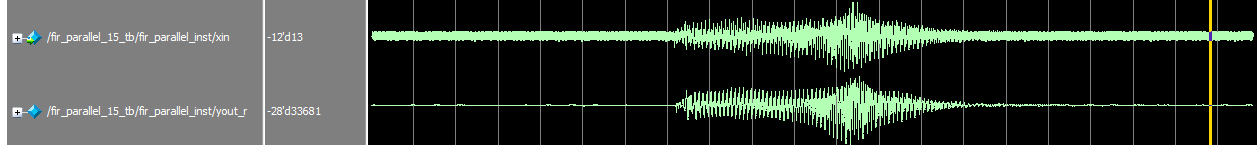
\includegraphics[width=0.7\textwidth]{image/2024-06-26-20-09-26.png}
    \caption{滤波结果仿真}
    \label{image_improve_sim_1_1}
\end{figure}
\begin{figure}[H]
    \centering
    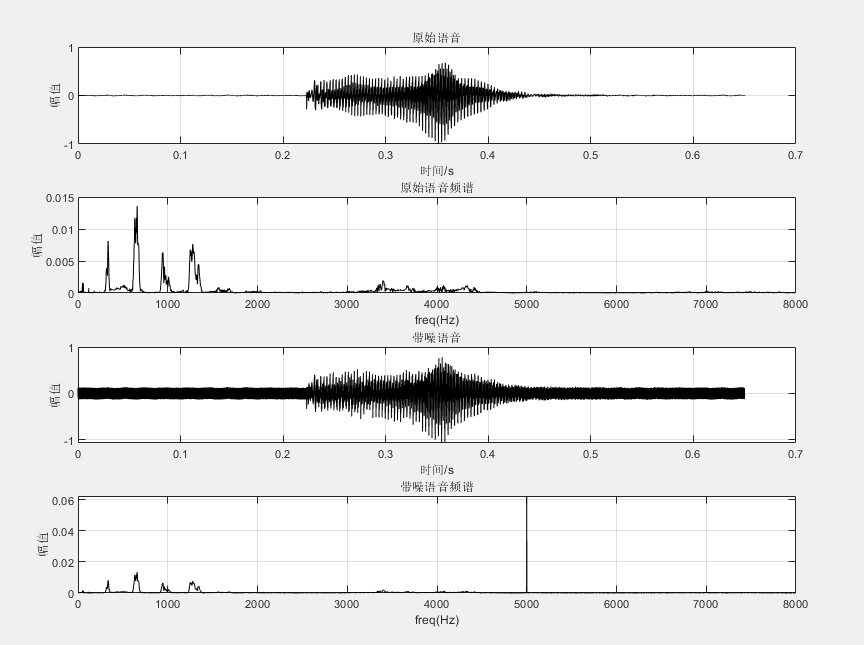
\includegraphics[width=0.7\textwidth]{image/2024-06-26-20-11-58.png}
    \caption{音频信号理论情况}
    \label{image_improve_sim_1_2}
\end{figure}
对输入信号, 即添加单频噪声的音频信号, 其时域图和频域图如图\ref{image_improve_sim_1_2}所示, 
滤波结果仿真如图\ref{image_improve_sim_1_1}所示, 可以看到滤波结果的时域非常接近原始音频信号, 
成功将音频信号中添加的单频噪声滤除。
\begin{figure}[H]
    \centering
    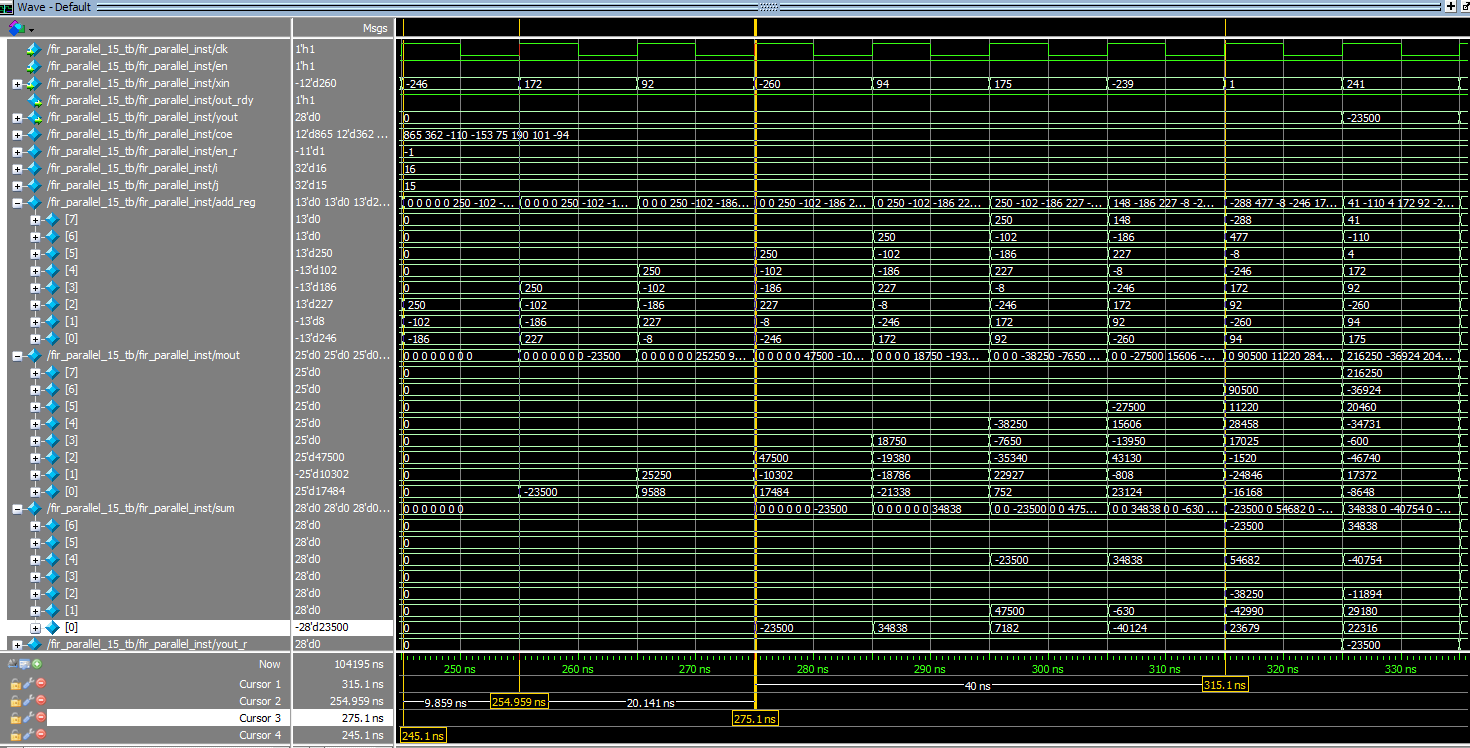
\includegraphics[width=0.7\textwidth]{image/2024-06-26-20-38-56.png}
    \caption{数据流仿真}
    \label{image_improve_sim_2}
\end{figure}
针对数据流的仿真如图\ref{image_improve_sim_2}所示, 从输入数据开始, 延迟两个时钟后, 得到add\_reg中的结果, 
之后延迟三个时钟后乘法器完成输出, 最后的累加积分的加法器也进行了优化, 因为使用了三级的延迟两个时钟的DSP Slice
中的加法器单元, 累加求和延迟6个时钟, 整套计算系统为流水线模式, 经过11个时钟后, 流水线被填满之后, 每个时钟输出
一个有效数据。
\subsection*{拓展任务}
\begin{figure}[H]
    \centering
    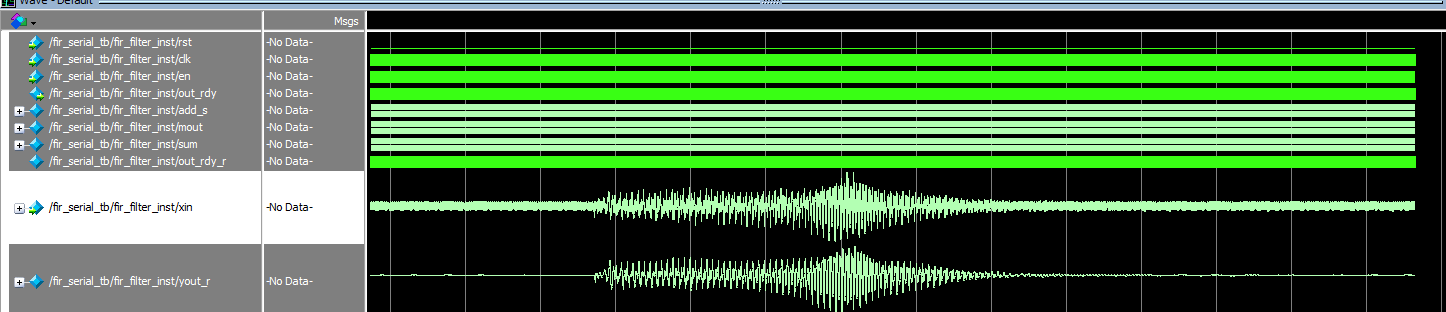
\includegraphics[width=0.7\textwidth]{image/2024-06-27-02-14-26.png}
    \caption{仿真效果图}
    \label{image_extend_sim_1}
\end{figure}
滤波效果仿真结果如图\ref{image_extend_sim_1}所示, 滤波效果理想, 可以看到加噪信号中的单频噪声被滤除。
\begin{figure}[H]
    \centering
    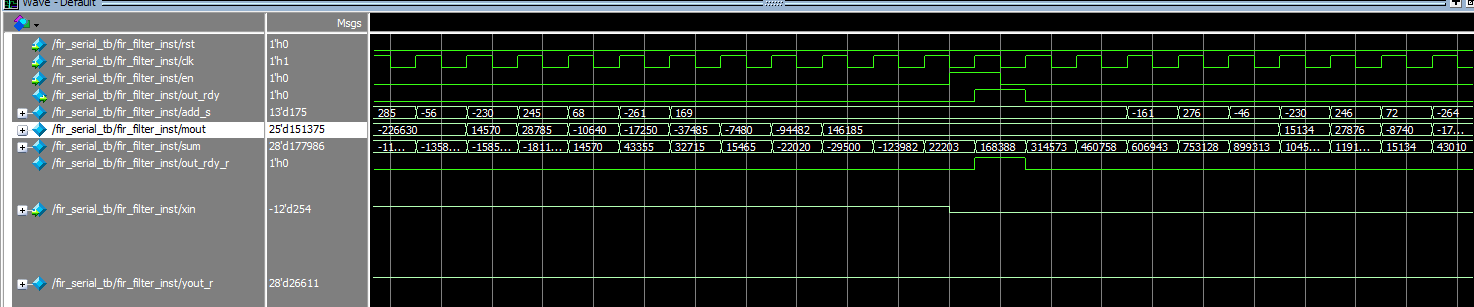
\includegraphics[width=0.7\textwidth]{image/2024-06-27-02-15-54.png}
    \caption{时序仿真图}
    \label{image_extend_sim_2}
\end{figure}

串行设计的FIR滤波器时序仿真如图\ref{image_extend_sim_2}所示, 可以看到其与并行设计的最大差异也直接体现在仿真上, 
不同的计算结果在并行FIR滤波器中体现为不同的数据, 不同的连线, 而在串行设计中只需要用到一个加法器, 一个乘法器和一
个累加器, 计算过程中的8次加法通过时分复用同一个模块实现, 因此导致了较长的计算延迟, 使用8个时钟计算一次数据输出。
图\ref{image_extend_sim_2}中可以看到, 不同的时钟周期, 模块的输出都不同, 而这些不同的数据属于一次计算, 最终比对
计算结果, 可以看到其计算结果与并行设计的相同系数的FIR数值一样。
% 第四部分
\subsection*{创新设计}
\begin{figure}[H]
    \centering
    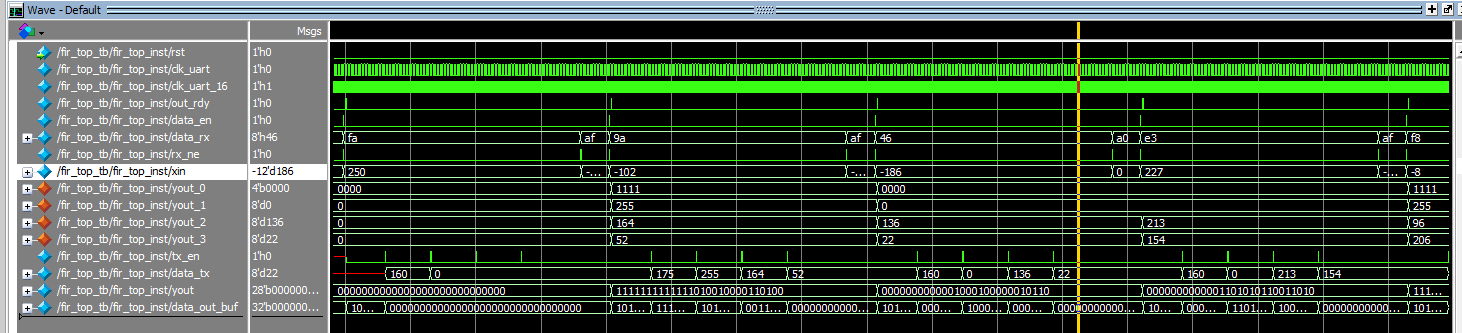
\includegraphics[width=0.7\textwidth]{image/2024-06-27-22-24-29.png}
    \caption{创新设计的仿真结果}
    \label{image_innovation_sim_1}
\end{figure}
创新设计部分的仿真结果如图\ref{image_innovation_sim_1}所示, 可以看到数据通过
串口发送到该模块后, 控制电路部分会等待有起始信号1010的数据, 同步输入数据, 每接
收到两个数据有效数据后, 去除1010标识符后送入FIR滤波器, 当FIR滤波器输出时, 将数
据缓存, 分8个bit通过串口的tx模块发送, 当上位机接收后, 再次传入数据, 之后计算完毕。
\section*{\fourhao 四、Matlab验证结果}
\xiaosihao
\setstretch{1.5}
% 记录加编程器与拨码开关和发光二极管、数码管等的连接情况。记录开发板硬件验证结果,并分析其结果的正确性。
% 按照基础任务、提高任务和拓展任务分别分析
\subsection*{基础任务}
使用Matlab进行验证的程序如下:
\begin{lstlisting}[language=Matlab, caption={基础任务Matlab验证结果}]
clear all; clc; close all;
fs = 5e3;
T = 1 / fs;
n = 0:2047;
t = n * T;
x = cos(2*pi*50*t) + 0.5*cos(2*pi*2000*t);
x = mapminmax(x);
x_dis = floor((2 ^ 11 - 1) * x);

b = [-137   -40   249   580   726   580   249   -40  -137];

x = x_dis;
y = round(filter(b, 1, x_dis));
time = t;
N = 2048;
% 读取FPGA滤波结果数据z
load res.mat
z = VarName1;
% 作图
subplot 611; plot(time,x,'k'); grid;
title('原始信号'); ylabel('幅值'); xlabel('时间/s');

subplot 612; audioFFT = fft(x);
plot((0:round(N/2)-1) / N * fs, abs(audioFFT(1:round(N/2)) / N), 'k');grid;
title('原始信号频谱'); ylabel('幅值'); xlabel('freq(Hz)');

subplot 613; plot(time,y,'k');grid;
title('Matlab滤波时域'); ylabel('幅值'); xlabel('时间/s');

subplot 614; audioFFT = fft(y);
plot((0:round(N/2)-1) / N * fs, abs(audioFFT(1:round(N/2)) / N), 'k');grid;
title('Maltab滤波频域'); ylabel('幅值'); xlabel('freq(Hz)');

subplot 615; plot(time,z,'k'); grid;
title('FPGA滤波后时域'); ylabel('幅值'); xlabel('时间/s');

subplot 616; audioFFT = fft(z);
plot((0:round(N/2)-1) / N * fs, abs(audioFFT(1:round(N/2)) / N), 'k');grid;
title('FPGA滤波后频域'); ylabel('幅值'); xlabel('freq(Hz)');
\end{lstlisting}
\begin{figure}[htbp]
    \centering
    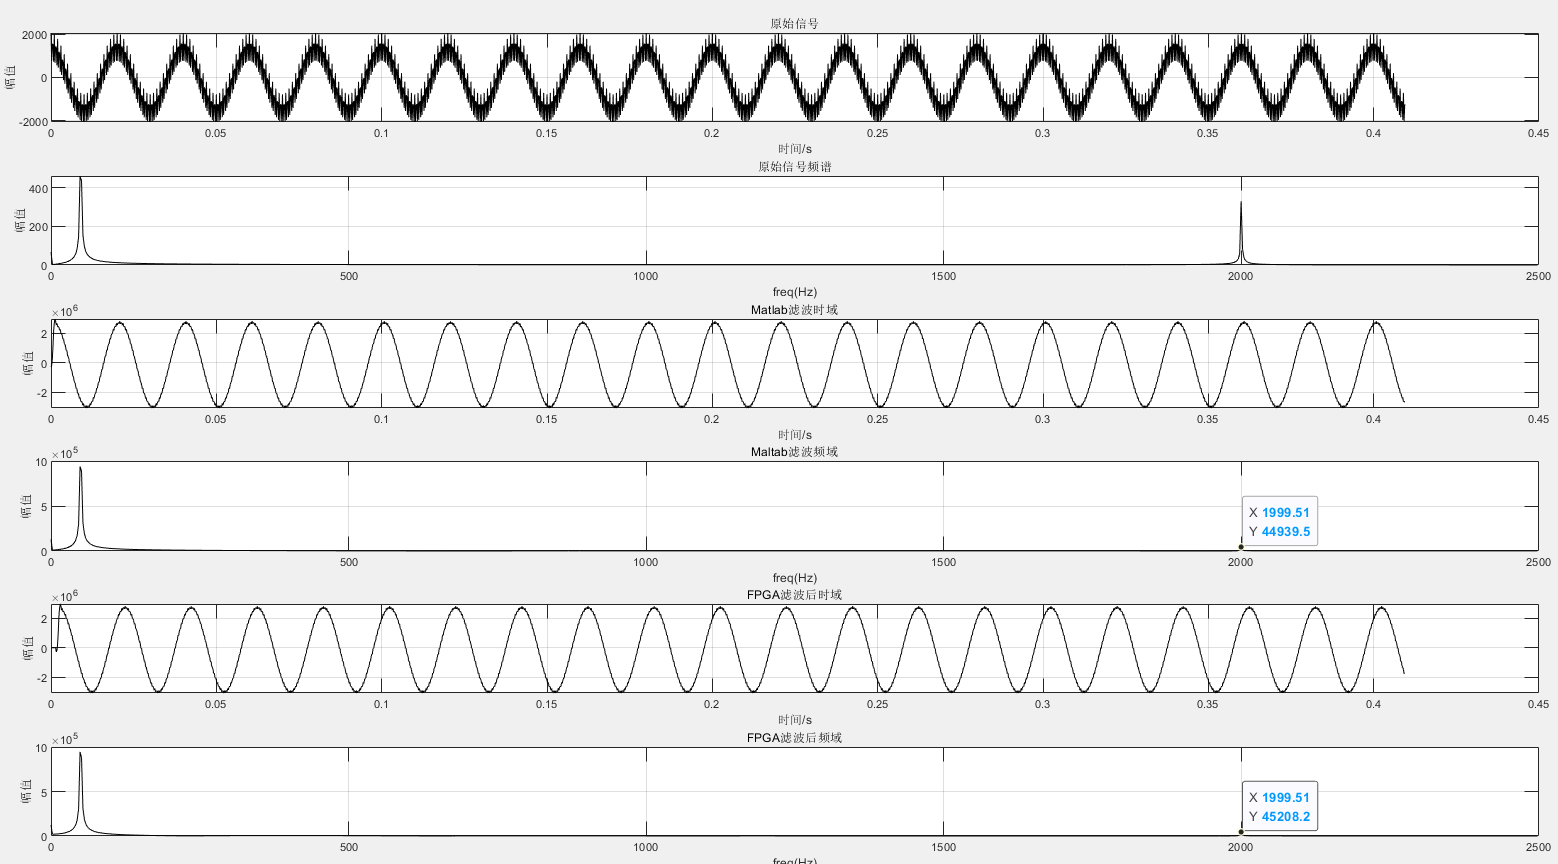
\includegraphics[width=0.7\textwidth]{image/2024-06-28-21-18-48.png}
    \caption{8阶并行FIR滤波器滤波结果}
    \label{image_verify_base_1}
\end{figure}
通过Matlab计算比对滤波结果, 结果如图\ref{image_verify_base_1}所示, FIR低通滤波器的效果基本实现, 
其中数据略微不同是由于FPGA滤波器将开始滤波时的无效数据输出, 导致了二者微小的差距。
\subsection*{提高任务}
\begin{figure}[H]
    \centering
    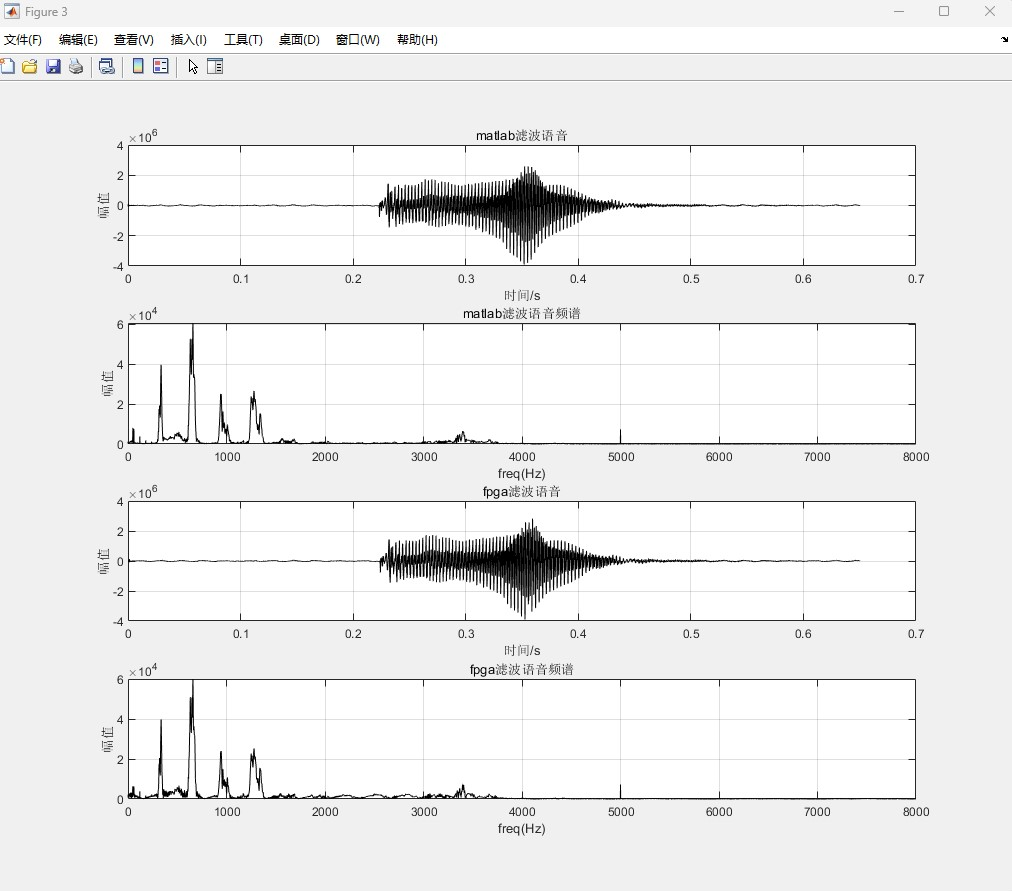
\includegraphics[width=0.7\textwidth]{image/2024-06-28-18-52-58.png}
    \caption{Matlab验证结果}
    \label{image_verify_improve_1}
\end{figure}
通过Matlab将计算结果比对, 结果如图\ref{image_verify_improve_1}所示, 效果很好的实现, 
可以从途中观察到数值有略微差距, 通过分析FPGA仿真输出的数据可以发现问题, 在进行数据输入
前, 数据输入使能便已经置位, 导致输出数据有一部分前导零, 采样固定点数截止便会导致会丢失
末尾几个滤波结果, 导致了滤波结果的细微差异。
\subsection*{拓展任务}
15阶滤波器对语音信号的Matlab滤波结果验证程序如下:
\begin{lstlisting}[language=Matlab, caption={语音信号滤波验证程序}]
[file, path]  = uigetfile('*.wav');     % 读取音频
[xx, fs] = audioread([path, file]);     % 读取音频

xx=xx-mean(xx);                         % 消除直流分量
x=xx/max(abs(xx));                      % 幅值归一化
N=length(x);                            % 计算音频长度

time=(0:N-1)/fs;                        % 计算时间
noiseFreq=5000;                         % 单频噪声频率
noiseAmp=0.125;                         % 单频噪声幅度
signal=x + noiseAmp*cos(2*pi*noiseFreq*time)';      % 添加噪声
x_dis = floor((2 ^ 11 - 1) * mapminmax(signal));    % 引入量化噪声
b = [-94   101   190    75  -153  -110   362   865   865   362  -110  -153    75   190   101   -94];
x = mapminmax(x_dis);
x = filter(b, 1, x);

load('res.mat');
y = mapminmax(res);
% 作图
subplot 411; plot(time,x,'k'); grid;
title('Matlab滤波信号时域'); ylabel('幅值'); xlabel('时间/s');

subplot 412; audioFFT = fft(x);
plot((0:round(N/2)-1) / N * fs, abs(audioFFT(1:round(N/2)) / N), 'k');grid;
title('Matlab滤波信号频域'); ylabel('幅值'); xlabel('freq(Hz)');

subplot 413; plot(time,y,'k');grid;
title('FPGA滤波时域'); ylabel('幅值'); xlabel('时间/s');

subplot 414; audioFFT = fft(y);
plot((0:round(N/2)-1) / N * fs, abs(audioFFT(1:round(N/2)) / N), 'k');grid;
title('FPGA滤波频域'); ylabel('幅值'); xlabel('freq(Hz)');    
\end{lstlisting}
\begin{figure}[H]
    \centering
    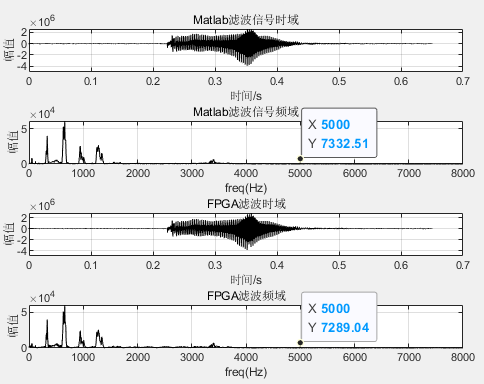
\includegraphics[width=0.7\textwidth]{image/2024-06-27-02-35-01.png}
    \caption{15阶串行FIR滤波器验证结果}
    \label{image_verify_extend_1}
\end{figure}
15阶串行FIR的滤波结果与15阶并行的FIR滤波器滤波结果一致, 相比之下没有并行FIR滤波器输出
的无效数据, 其值更加接近Matlab的滤波结果, 认为二者效果相同, 从图中也可以明显的观察到信
号为发生相位失真, 具备FIR滤波器的特性。
% 第五部分
\section*{\fourhao 五、创新内容的硬件验证结果}
\xiaosihao
\setstretch{1.5}
\begin{figure}[H]
    \centering
    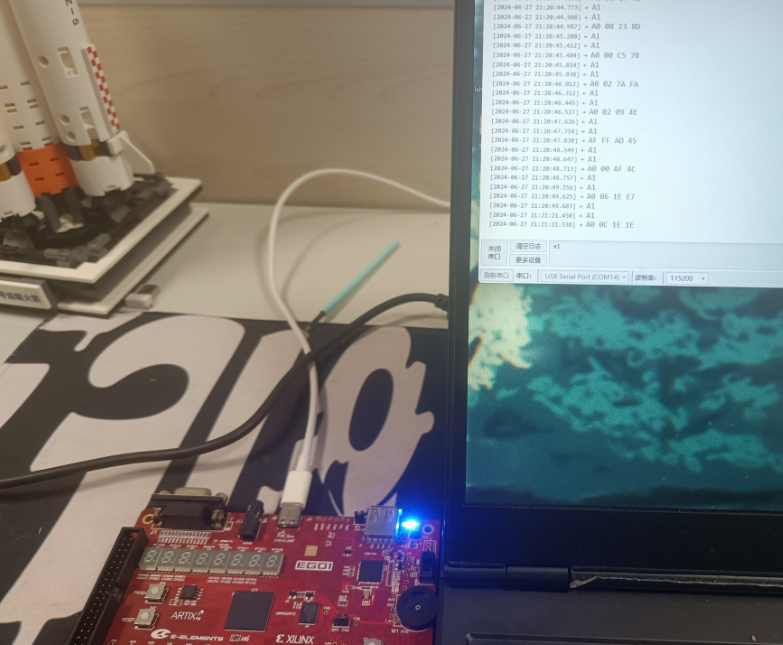
\includegraphics[width=0.7\textwidth]{image/2024-06-27-21-22-24.png}
    \caption{基于串口的FIR滤波器设计验证实验结果}
    \label{image_verify_hardware_1}
\end{figure}
串口FIR硬件效果如图\ref{image_verify_hardware_1}所示, 输入数据为12bit, 输出数据为28bit, 
串口使用8bit进行通信, 在输入数据和输出数据前添加4bit的前同步码, "1010", 即图\ref{image_verify_hardware_1}中串口调
试助手显示的十六进制数据0xA,PC上位机向FPGA传输两个数据后, 输入数据达到12bit, 进行一次计算, 输出4个8bit结果, 其中包含
28bit数据。\\

针对创新部分的串口硬件验证过程, 设计MATLAB脚本程序, 通过串口实现FIR滤波, 其程序如下:
\begin{lstlisting}[language=Matlab, caption={Matlab通过串口与FPGA的FIR传输数据并验证}]
clear all;
hserial = serialport("COM14", 115200, "ByteOrder", "big-endian");
flush(hserial);

[file, path]  = uigetfile('*.wav');             % 读取音频
[xx, fs] = audioread([path, file]);             % 读取音频

xx = xx-mean(xx);                               % 消除直流分量
x = xx/max(abs(xx));                            % 幅值归一化
N = length(x);                                  % 计算音频长度
time=(0:N-1)/fs;                                % 计算时间
noiseFreq=5000;                                 % 单频噪声频率
noiseAmp=0.125;                                 % 单频噪声幅度
signal=x + noiseAmp*cos(2*pi*noiseFreq*time)';  % 添加噪声

q_12 = quantizer('Format', [12, 0]);
res = mapminmax(signal);                        % 归一化数据
x_dis_1 = floor((2 ^ 11 - 1) * res);            % 数据量化
x_dis_2 = num2bin(q_12, x_dis_1);
x_dis_bin = strcat(repmat("1010", N, 1), x_dis_2);   % 添加1010标识

q_8 = quantizer('Format', [8, 0], 'DataMode', 'ufixed');
q_32 = quantizer('Format', [32, 0]);
signal_filtered = zeros(1, N);
for index = 1:N
    str = x_dis_bin(index);
    data_out = bin2num(q_8, extractBefore(str, 9));
    write(hserial, data_out, "uint8");
    data_out = bin2num(q_8, extractAfter(str, 8));
    write(hserial, data_out, "uint8");
    data = read(hserial, 1, "uint32");
    % 符号位扩展
    for k = 0:3
        data = bitset(data, 32-k, bitget(data, 28));
    end
    % 识别补码, 转化为符号数输出
    signal_filtered(index) = bin2num(q_32, dec2bin(data));
end
save result
% load result.mat
% 作图
xx = signal - mean(signal);
signal = xx/max(abs(xx));
xx = signal_filtered - mean(signal_filtered);
signal_filtered = xx/max(abs(xx));
subplot 611; plot(time,x,'k'); grid;
title('原始语音'); ylabel('幅值'); xlabel('时间/s');

subplot 612; audioFFT = fft(x);
plot((0:round(N/2)-1) / N * fs, abs(audioFFT(1:round(N/2)) / N), 'k');grid;
title('原始语音频谱'); ylabel('幅值'); xlabel('freq(Hz)');

subplot 613; plot(time,signal,'k');grid;
title('带噪语音'); ylabel('幅值'); xlabel('时间/s');

subplot 614; audioFFT = fft(signal);
plot((0:round(N/2)-1) / N * fs, abs(audioFFT(1:round(N/2)) / N), 'k');grid;
title('带噪语音频谱'); ylabel('幅值'); xlabel('freq(Hz)');

subplot 615; plot(time,signal_filtered,'k'); grid;
title('FPGA滤波后时域'); ylabel('幅值'); xlabel('时间/s');

subplot 616; audioFFT = fft(signal_filtered);
plot((0:round(N/2)-1) / N * fs, abs(audioFFT(1:round(N/2)) / N), 'k');grid;
title('FPGA滤波后频域'); ylabel('幅值'); xlabel('freq(Hz)');
\end{lstlisting}
\begin{figure}[H]
    \centering
    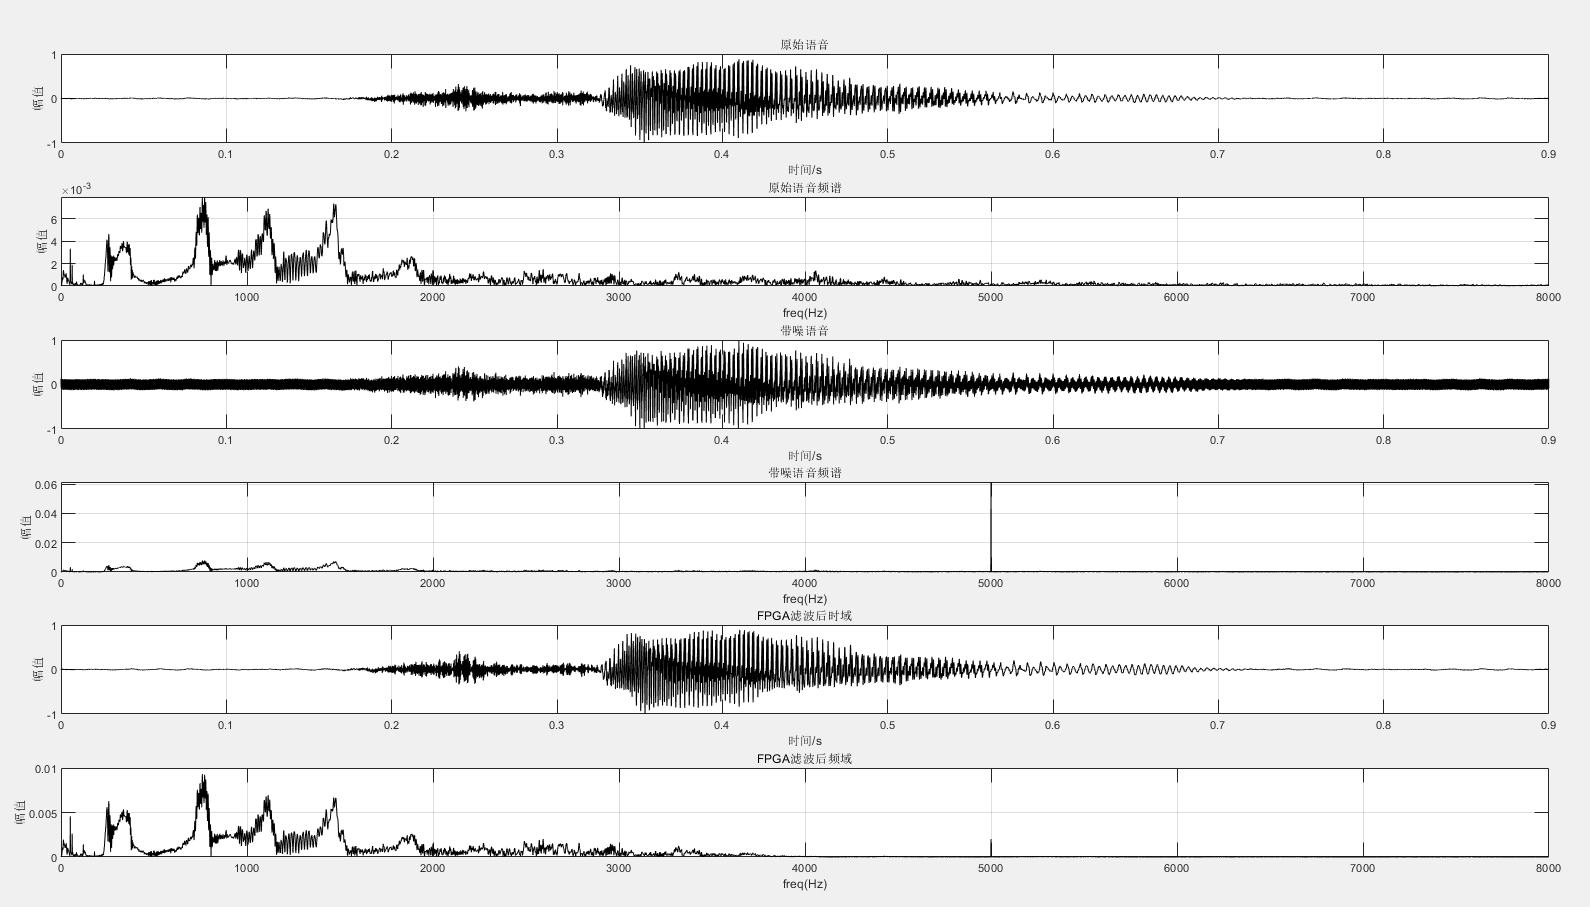
\includegraphics[width=0.7\textwidth]{image/2024-06-27-21-57-44.png}
    \caption{FPGA硬件验证结果}
    \label{image_verify_hardware_2}
\end{figure}
通过串口将待滤波数据传输到FPGA开发板上, 并通过串口读取其回传的滤波结果, 之后绘制
其时域和频域图, 得到如图\ref{image_verify_hardware_2}所示的结果, 改滤波器的效果显著, 
且无线性相位失真发生, 效果明显, 证明了在提高任务和拓展任务中使用xilinx提供的DSP48E的
IP核设计的FIR滤波器可以在硬件上有效的工作, 不仅仅局限于仿真结果。
\section*{\fourhao 六、问题解决}
\xiaosihao
\setstretch{1.5}
% 设计过程中遇到的问题及解决的方法。
\subsection*{Vivado的仿真过程中经常出现UI问题}
解决: Vivado的仿真界面虽然美观但是经常出现波形上数字消失, 而且模拟波形可以随意放缩比例尺, 不利于固定图像比例比对不同波形, 
不利于观察波形, 最后简单的仿真过程, 如本次设计中的简单时序问题通过Vivado仿真, 但是复杂的如模拟波形数据, 流水线数据等通过Modelsim进行仿真。
\subsection*{Modelsim和Vivado的联合仿真, 在修改文件后需要重启}
解决: 通过查阅资料查看原理, 了解到Vivado在调用Modelsim仿真时是将文件交付Modelsim后, 其会对仿真文件和源文件进行编译, 然后再进行仿真, 
并且编译结果是静态的, 仅仅重新编译还不够, 还需要手动更新。Vivado交付给Modelsim的源文件保存在Modelsim中的xil\_defaultlib库中, 更改文
件后找到对应文件update以后再进行recompile, 之后reset仿真, 再次仿真就是更改后的仿真结果。 
\subsection*{串行FIR滤波器的设计过程无论如何改动, 结果都不正确}
解决: 花费很长的时间观察仿真时序图, 起初未考虑到加法器的2周期时延与滤波器系数直接赋值无时延导致的不同步,
一直认为是累加器的累加过程中BYPASS信号控制不正确, 最后实在无法定位问题, 信号输入开始, 通过笔算的形式手动计
算FIR结果和流程, 最终将问题定位到滤波器系数提前加法器输出两个周期的问题, 通过缓存移位寄存器人为将滤波器系数
的赋值延迟2个周期, 解决问题, 最终得到与并行FIR滤波器完全一致的计算结果。
% 第六部分
\section*{\fourhao 七、心得体会}
\xiaosihao
\setstretch{1.5}
作为最后的创新设计实验, 追求创新的前提下是比综合设计更加进一步复杂的设计过程。在本次创新设计中由于设计的是FIR滤波器,
相比于乘法器或者求解最大公倍数等等简单的算法而言, FIR滤波器的算法原理上不复杂, 但随着阶数的上升其结构会极度的复杂。\\

如果直接在算法中使用"*"或者"+"会使得设计过程十分简单, 但如果通过仿真的方式验证的话, 仿真工具不会考虑乘法和加法得综合结果, 
直接以计算机语言得形式进行计算仿真, 只要结构正确, 就可以得到正确的结果, 此外, 直接使用*和+的综合结果是未知的, 
在未指定的情况下, 甚至无法正确处理符号数\\

在实际的设计中, 会使用并行或者串行加上流水线形式得乘法器和加法器进行设计。比如,对滤波器输出得最后累加积分过程中, 
并行设计的输出如果直接使用7个"+"将8个数据相加, 综合工具甚至会将该累加过程综合成"一群"LUT构成的组合逻辑, 在实际应
用中如此庞大得组合逻辑电路肯定无法完全避免竞争冒险等毛刺问题, 以至于最终设计得到得FIR滤波器只能在很低的工作频率下
运行, 甚至有可能出错。由于创新设计得时间有限, 采用Xilinx FPGA上集成的DSP模块中的乘法器和累加器实现FIR滤波器, 实现
设计安全和高效的均衡。\\

在设计阶段, 花费了将近3/4的时间用于仿真, 仿真能力得到了极大的提升, 从最开始的找不到仿真方向, 到现在可以熟练的联合Matlab和
Modelsim等仿真工具, 熟悉了Verilog仿真文件中的若干系统级函数, 也对Modelsim仿真工具更加熟练。\\

最后不满足于仅仅通过仿真实现FIR滤波器, 尝试在硬件上验证所设计FIR滤波器的有效性, 但局限于信号发生器、示波器等的设备问题, 
放弃了XADC采样信号的并通过DAC再生的验证思路, 着眼于使用串口将FPGA与上位机连接, FPGA作为一个独立的计算单元供上位机调用, 
上位机通过Matalb程序验证FPGA输出的计算结果是否正确。在该创新内容的设计过程中, 掌握了很多新的能力,如Matlab对系统串口资
源的使用, Matlab中补码的整数的转换等, 以及更加复杂的仿真文件的编写等。\\

通过对数字滤波器和Matlab的设计, 不仅加深了自己对于FPGA技术的理解, 同时巩固了自己所学过的理论知识。
\end{document}
